\documentclass[twoside]{book}

% Packages required by doxygen
\usepackage{calc}
\usepackage{doxygen}
\usepackage{graphicx}
\usepackage[utf8]{inputenc}
\usepackage{makeidx}
\usepackage{multicol}
\usepackage{multirow}
\usepackage{textcomp}
\usepackage[table]{xcolor}

% Font selection
\usepackage[T1]{fontenc}
\usepackage{mathptmx}
\usepackage[scaled=.90]{helvet}
\usepackage{courier}
\usepackage{amssymb}
\usepackage{sectsty}
\renewcommand{\familydefault}{\sfdefault}
\allsectionsfont{%
  \fontseries{bc}\selectfont%
  \color{darkgray}%
}
\renewcommand{\DoxyLabelFont}{%
  \fontseries{bc}\selectfont%
  \color{darkgray}%
}

% Page & text layout
\usepackage{geometry}
\geometry{%
  a4paper,%
  top=2.5cm,%
  bottom=2.5cm,%
  left=2.5cm,%
  right=2.5cm%
}
\tolerance=750
\hfuzz=15pt
\hbadness=750
\setlength{\emergencystretch}{15pt}
\setlength{\parindent}{0cm}
\setlength{\parskip}{0.2cm}
\makeatletter
\renewcommand{\paragraph}{%
  \@startsection{paragraph}{4}{0ex}{-1.0ex}{1.0ex}{%
    \normalfont\normalsize\bfseries\SS@parafont%
  }%
}
\renewcommand{\subparagraph}{%
  \@startsection{subparagraph}{5}{0ex}{-1.0ex}{1.0ex}{%
    \normalfont\normalsize\bfseries\SS@subparafont%
  }%
}
\makeatother

% Headers & footers
\usepackage{fancyhdr}
\pagestyle{fancyplain}
\fancyhead[LE]{\fancyplain{}{\bfseries\thepage}}
\fancyhead[CE]{\fancyplain{}{}}
\fancyhead[RE]{\fancyplain{}{\bfseries\leftmark}}
\fancyhead[LO]{\fancyplain{}{\bfseries\rightmark}}
\fancyhead[CO]{\fancyplain{}{}}
\fancyhead[RO]{\fancyplain{}{\bfseries\thepage}}
\fancyfoot[LE]{\fancyplain{}{}}
\fancyfoot[CE]{\fancyplain{}{}}
\fancyfoot[RE]{\fancyplain{}{\bfseries\scriptsize Generated on Sat Mar 29 2014 16\-:54\-:10 for Form Manager by Doxygen }}
\fancyfoot[LO]{\fancyplain{}{\bfseries\scriptsize Generated on Sat Mar 29 2014 16\-:54\-:10 for Form Manager by Doxygen }}
\fancyfoot[CO]{\fancyplain{}{}}
\fancyfoot[RO]{\fancyplain{}{}}
\renewcommand{\footrulewidth}{0.4pt}
\renewcommand{\chaptermark}[1]{%
  \markboth{#1}{}%
}
\renewcommand{\sectionmark}[1]{%
  \markright{\thesection\ #1}%
}

% Indices & bibliography
\usepackage{natbib}
\usepackage[titles]{tocloft}
\setcounter{tocdepth}{3}
\setcounter{secnumdepth}{5}
\makeindex

% Hyperlinks (required, but should be loaded last)
\usepackage{ifpdf}
\ifpdf
  \usepackage[pdftex,pagebackref=true]{hyperref}
\else
  \usepackage[ps2pdf,pagebackref=true]{hyperref}
\fi
\hypersetup{%
  colorlinks=true,%
  linkcolor=blue,%
  citecolor=blue,%
  unicode%
}

% Custom commands
\newcommand{\clearemptydoublepage}{%
  \newpage{\pagestyle{empty}\cleardoublepage}%
}


%===== C O N T E N T S =====

\begin{document}

% Titlepage & ToC
\hypersetup{pageanchor=false}
\pagenumbering{roman}
\begin{titlepage}
\vspace*{7cm}
\begin{center}%
{\Large Form Manager \\[1ex]\large Beta Ver. 2.\-0 }\\
\vspace*{1cm}
{\large Generated by Doxygen 1.8.6}\\
\vspace*{0.5cm}
{\small Sat Mar 29 2014 16:54:10}\\
\end{center}
\end{titlepage}
\clearemptydoublepage
\tableofcontents
\clearemptydoublepage
\pagenumbering{arabic}
\hypersetup{pageanchor=true}

%--- Begin generated contents ---
\chapter{Hierarchical Index}
\section{Class Hierarchy}
This inheritance list is sorted roughly, but not completely, alphabetically\-:\begin{DoxyCompactList}
\item \contentsline{section}{Fields}{\pageref{class_fields}}{}
\begin{DoxyCompactList}
\item \contentsline{section}{Date\-List}{\pageref{class_date_list}}{}
\item \contentsline{section}{Drop\-List}{\pageref{class_drop_list}}{}
\begin{DoxyCompactList}
\item \contentsline{section}{Country\-List}{\pageref{class_country_list}}{}
\end{DoxyCompactList}
\item \contentsline{section}{Html\-Text}{\pageref{class_html_text}}{}
\item \contentsline{section}{Text\-Input}{\pageref{class_text_input}}{}
\begin{DoxyCompactList}
\item \contentsline{section}{Text\-Box}{\pageref{class_text_box}}{}
\end{DoxyCompactList}
\item \contentsline{section}{Time\-List}{\pageref{class_time_list}}{}
\end{DoxyCompactList}
\item \contentsline{section}{Form}{\pageref{class_form}}{}
\item \contentsline{section}{Form\-Manager}{\pageref{class_form_manager}}{}
\item \contentsline{section}{Form\-Util}{\pageref{class_form_util}}{}
\end{DoxyCompactList}

\chapter{Data Structure Index}
\section{Data Structures}
Here are the data structures with brief descriptions\-:\begin{DoxyCompactList}
\item\contentsline{section}{\hyperlink{class_country_list}{Country\-List} \\*A special drop list for countries }{\pageref{class_country_list}}{}
\item\contentsline{section}{\hyperlink{class_date_list}{Date\-List} \\*A special drop list for dates to be used in \hyperlink{class_form}{Form} }{\pageref{class_date_list}}{}
\item\contentsline{section}{\hyperlink{class_drop_list}{Drop\-List} \\*Drop list field for \hyperlink{class_form}{Form} Used for drop down lists within html form }{\pageref{class_drop_list}}{}
\item\contentsline{section}{\hyperlink{class_fields}{Fields} \\*Abstract class for fields }{\pageref{class_fields}}{}
\item\contentsline{section}{\hyperlink{class_form}{Form} \\*A canvas for form field (components), form info, and display info }{\pageref{class_form}}{}
\item\contentsline{section}{\hyperlink{class_form_manager}{Form\-Manager} \\*Class for managing multiple forms }{\pageref{class_form_manager}}{}
\item\contentsline{section}{\hyperlink{class_form_util}{Form\-Util} \\*A static helper class for \hyperlink{class_form}{Form} related functions }{\pageref{class_form_util}}{}
\item\contentsline{section}{\hyperlink{class_html_text}{Html\-Text} \\*Contains html text to output in \hyperlink{class_form}{Form} }{\pageref{class_html_text}}{}
\item\contentsline{section}{\hyperlink{class_text_box}{Text\-Box} \\*Text box field for \hyperlink{class_form}{Form} }{\pageref{class_text_box}}{}
\item\contentsline{section}{\hyperlink{class_text_input}{Text\-Input} \\*Text input bar field for \hyperlink{class_form}{Form} }{\pageref{class_text_input}}{}
\item\contentsline{section}{\hyperlink{class_time_list}{Time\-List} \\*A special drop list for time to be used in \hyperlink{class_form}{Form} }{\pageref{class_time_list}}{}
\end{DoxyCompactList}

\chapter{Data Structure Documentation}
\hypertarget{class_country_list}{\section{Country\-List Class Reference}
\label{class_country_list}\index{Country\-List@{Country\-List}}
}


A special drop list for countries.  


Inheritance diagram for Country\-List\-:\begin{figure}[H]
\begin{center}
\leavevmode
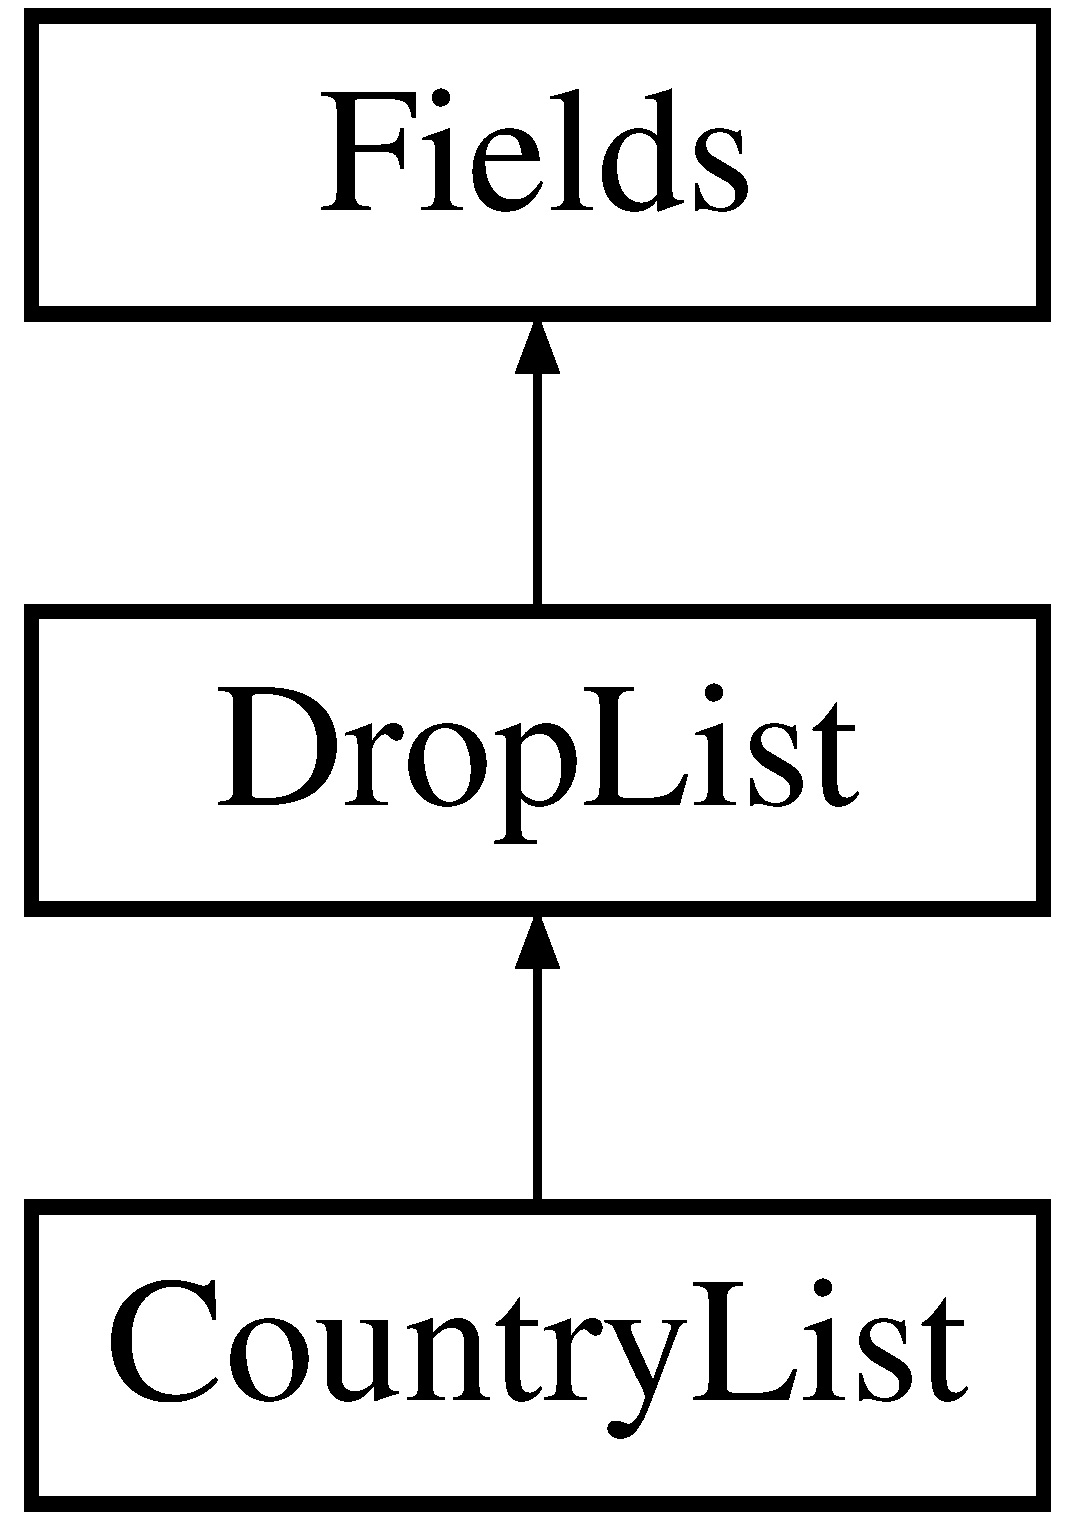
\includegraphics[height=3.000000cm]{class_country_list}
\end{center}
\end{figure}
\subsection*{Public Member Functions}
\begin{DoxyCompactItemize}
\item 
\hyperlink{class_country_list_ac610fc08cbb0781b26136636de129bc0}{\-\_\-\-\_\-construct} (\$nm)
\begin{DoxyCompactList}\small\item\em Constructor for class. \end{DoxyCompactList}\end{DoxyCompactItemize}
\subsection*{Additional Inherited Members}


\subsection{Detailed Description}
A special drop list for countries. 

Essentially a pre-\/defined drop list with preloaded countries list hard coded into the script. Please note that it extends \hyperlink{class_drop_list}{Drop\-List}, as such, options can be added or removed. Also, Countries are in alphabetical order except for U.\-S. where it is first. (May be deprecated) Bug\-: Set default does not seem to work as of Beta Ver. 1.\-4 

\subsection{Constructor \& Destructor Documentation}
\hypertarget{class_country_list_ac610fc08cbb0781b26136636de129bc0}{\index{Country\-List@{Country\-List}!\-\_\-\-\_\-construct@{\-\_\-\-\_\-construct}}
\index{\-\_\-\-\_\-construct@{\-\_\-\-\_\-construct}!CountryList@{Country\-List}}
\subsubsection[{\-\_\-\-\_\-construct}]{\setlength{\rightskip}{0pt plus 5cm}\-\_\-\-\_\-construct (
\begin{DoxyParamCaption}
\item[{}]{\$nm}
\end{DoxyParamCaption}
)}}\label{class_country_list_ac610fc08cbb0781b26136636de129bc0}


Constructor for class. 

Requires unique name to be used in field, html name attribute, and Forms. 

The documentation for this class was generated from the following file\-:\begin{DoxyCompactItemize}
\item 
Form.\-php\end{DoxyCompactItemize}

\hypertarget{class_date_list}{\section{Date\-List Class Reference}
\label{class_date_list}\index{Date\-List@{Date\-List}}
}


A special drop list for dates to be used in \hyperlink{class_form}{Form}.  


Inheritance diagram for Date\-List\-:\begin{figure}[H]
\begin{center}
\leavevmode
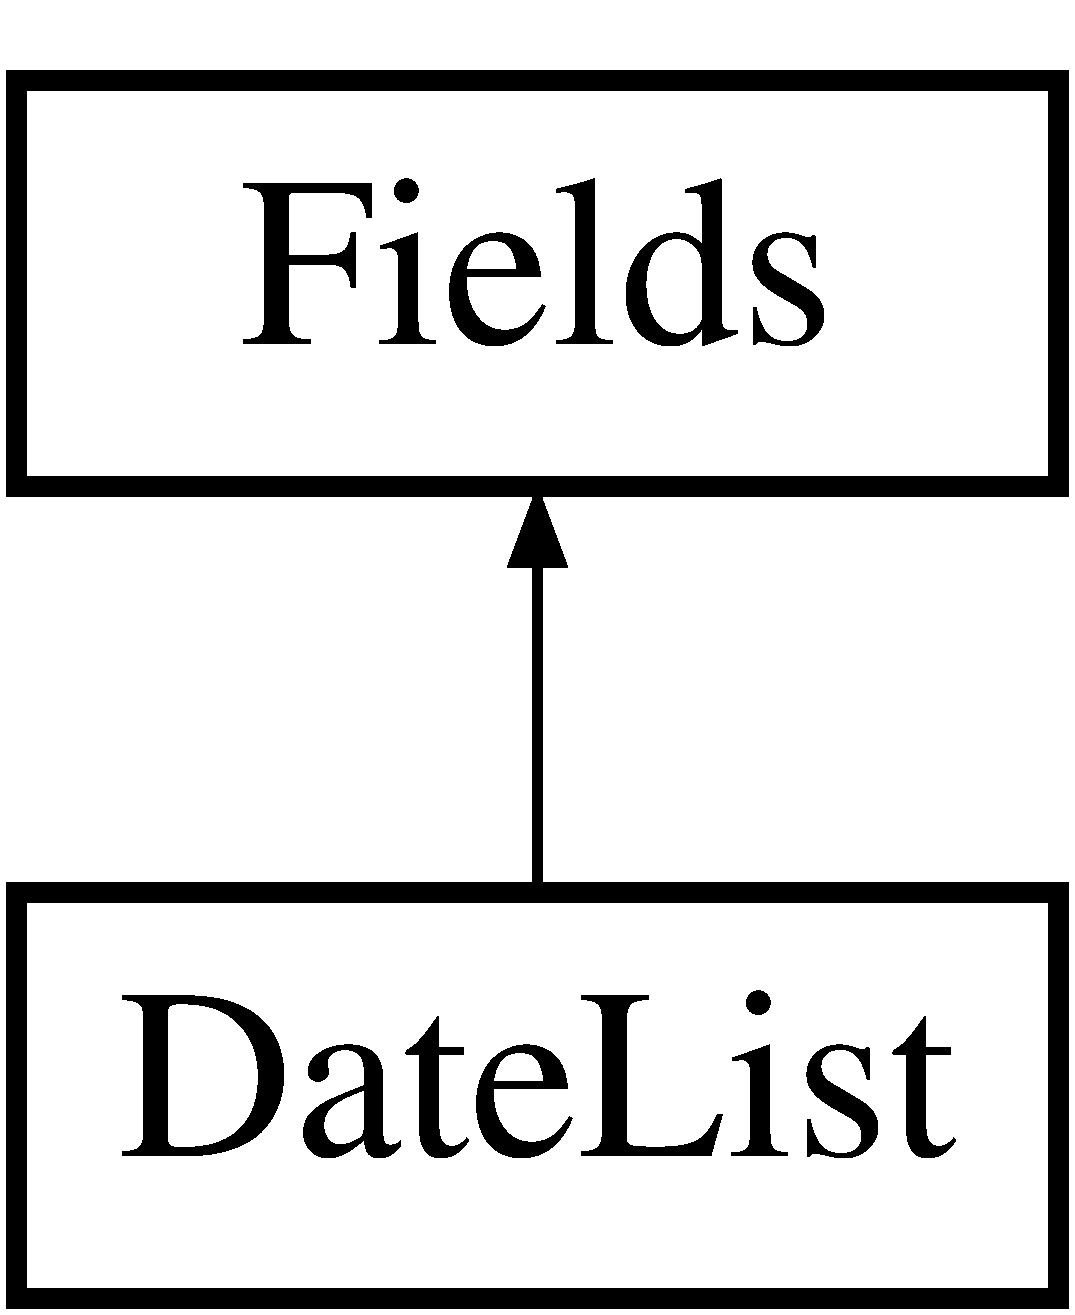
\includegraphics[height=2.000000cm]{class_date_list}
\end{center}
\end{figure}
\subsection*{Public Member Functions}
\begin{DoxyCompactItemize}
\item 
\hyperlink{class_date_list_ac610fc08cbb0781b26136636de129bc0}{\-\_\-\-\_\-construct} (\$nm)
\begin{DoxyCompactList}\small\item\em Constructor for class. \end{DoxyCompactList}\item 
\hypertarget{class_date_list_a421831a265621325e1fdd19aace0c758}{\hyperlink{class_date_list_a421831a265621325e1fdd19aace0c758}{\-\_\-\-\_\-destruct} ()}\label{class_date_list_a421831a265621325e1fdd19aace0c758}

\begin{DoxyCompactList}\small\item\em Default de-\/constructor for class. \end{DoxyCompactList}\item 
\hypertarget{class_date_list_a6f75ffe7d98c9e375394d63f8d379b2d}{{\bfseries set\-Class} (\$nm)}\label{class_date_list_a6f75ffe7d98c9e375394d63f8d379b2d}

\item 
\hypertarget{class_date_list_a4e25c00802ca9e9afb52a9177014fea7}{{\bfseries set\-Div\-Class} (\$nm)}\label{class_date_list_a4e25c00802ca9e9afb52a9177014fea7}

\item 
\hypertarget{class_date_list_a24d89b0ad05ea2e33626b1fc8ed59bc3}{{\bfseries get\-Date} ()}\label{class_date_list_a24d89b0ad05ea2e33626b1fc8ed59bc3}

\item 
\hypertarget{class_date_list_adc30a2a4d3e48cb6aee21562afbc4022}{{\bfseries get\-Default} ()}\label{class_date_list_adc30a2a4d3e48cb6aee21562afbc4022}

\item 
\hyperlink{class_date_list_aaf2bb7deba74bb0f994044954bd74ff3}{set\-Default} (\$d)
\begin{DoxyCompactList}\small\item\em Set default for class value. \end{DoxyCompactList}\item 
\hyperlink{class_date_list_a14814e04b348120748912692645f3a75}{get\-Contents} ()
\begin{DoxyCompactList}\small\item\em Get the value of the field as html format. Used by form. \end{DoxyCompactList}\end{DoxyCompactItemize}
\subsection*{Private Member Functions}
\begin{DoxyCompactItemize}
\item 
\hypertarget{class_date_list_a85460a970770dab21ad47a84ae0954fd}{\hyperlink{class_date_list_a85460a970770dab21ad47a84ae0954fd}{format\-D\-List} (\$nm)}\label{class_date_list_a85460a970770dab21ad47a84ae0954fd}

\begin{DoxyCompactList}\small\item\em Private function to format and set up the three individual drop lists. \end{DoxyCompactList}\end{DoxyCompactItemize}
\subsection*{Additional Inherited Members}


\subsection{Detailed Description}
A special drop list for dates to be used in \hyperlink{class_form}{Form}. 

Class manages three drop lists\-: month, date, and year. The class acts accordingly and reacts like a single field. 

\subsection{Constructor \& Destructor Documentation}
\hypertarget{class_date_list_ac610fc08cbb0781b26136636de129bc0}{\index{Date\-List@{Date\-List}!\-\_\-\-\_\-construct@{\-\_\-\-\_\-construct}}
\index{\-\_\-\-\_\-construct@{\-\_\-\-\_\-construct}!DateList@{Date\-List}}
\subsubsection[{\-\_\-\-\_\-construct}]{\setlength{\rightskip}{0pt plus 5cm}\-\_\-\-\_\-construct (
\begin{DoxyParamCaption}
\item[{}]{\$nm}
\end{DoxyParamCaption}
)}}\label{class_date_list_ac610fc08cbb0781b26136636de129bc0}


Constructor for class. 

Requires unique name to be used in field, html name attribute, and Forms. 

\subsection{Member Function Documentation}
\hypertarget{class_date_list_a14814e04b348120748912692645f3a75}{\index{Date\-List@{Date\-List}!get\-Contents@{get\-Contents}}
\index{get\-Contents@{get\-Contents}!DateList@{Date\-List}}
\subsubsection[{get\-Contents}]{\setlength{\rightskip}{0pt plus 5cm}get\-Contents (
\begin{DoxyParamCaption}
{}
\end{DoxyParamCaption}
)}}\label{class_date_list_a14814e04b348120748912692645f3a75}


Get the value of the field as html format. Used by form. 

Default html names for the three drop lists are \$this-\/$>$name.'month' \$this-\/$>$name.'day' and \$this-\/$>$name.'year'. \hypertarget{class_date_list_aaf2bb7deba74bb0f994044954bd74ff3}{\index{Date\-List@{Date\-List}!set\-Default@{set\-Default}}
\index{set\-Default@{set\-Default}!DateList@{Date\-List}}
\subsubsection[{set\-Default}]{\setlength{\rightskip}{0pt plus 5cm}set\-Default (
\begin{DoxyParamCaption}
\item[{}]{\$d}
\end{DoxyParamCaption}
)}}\label{class_date_list_aaf2bb7deba74bb0f994044954bd74ff3}


Set default for class value. 

Default must be in format of 'm/d/\-Y' with month and day being two digits. Year being four. Slashes can also be '-\/' as they will be replaced automatically into '/'. 

The documentation for this class was generated from the following file\-:\begin{DoxyCompactItemize}
\item 
Form.\-php\end{DoxyCompactItemize}

\hypertarget{class_drop_list}{\section{Drop\-List Class Reference}
\label{class_drop_list}\index{Drop\-List@{Drop\-List}}
}


Drop list field for \hyperlink{class_form}{Form} Used for drop down lists within html form.  


Inheritance diagram for Drop\-List\-:\begin{figure}[H]
\begin{center}
\leavevmode
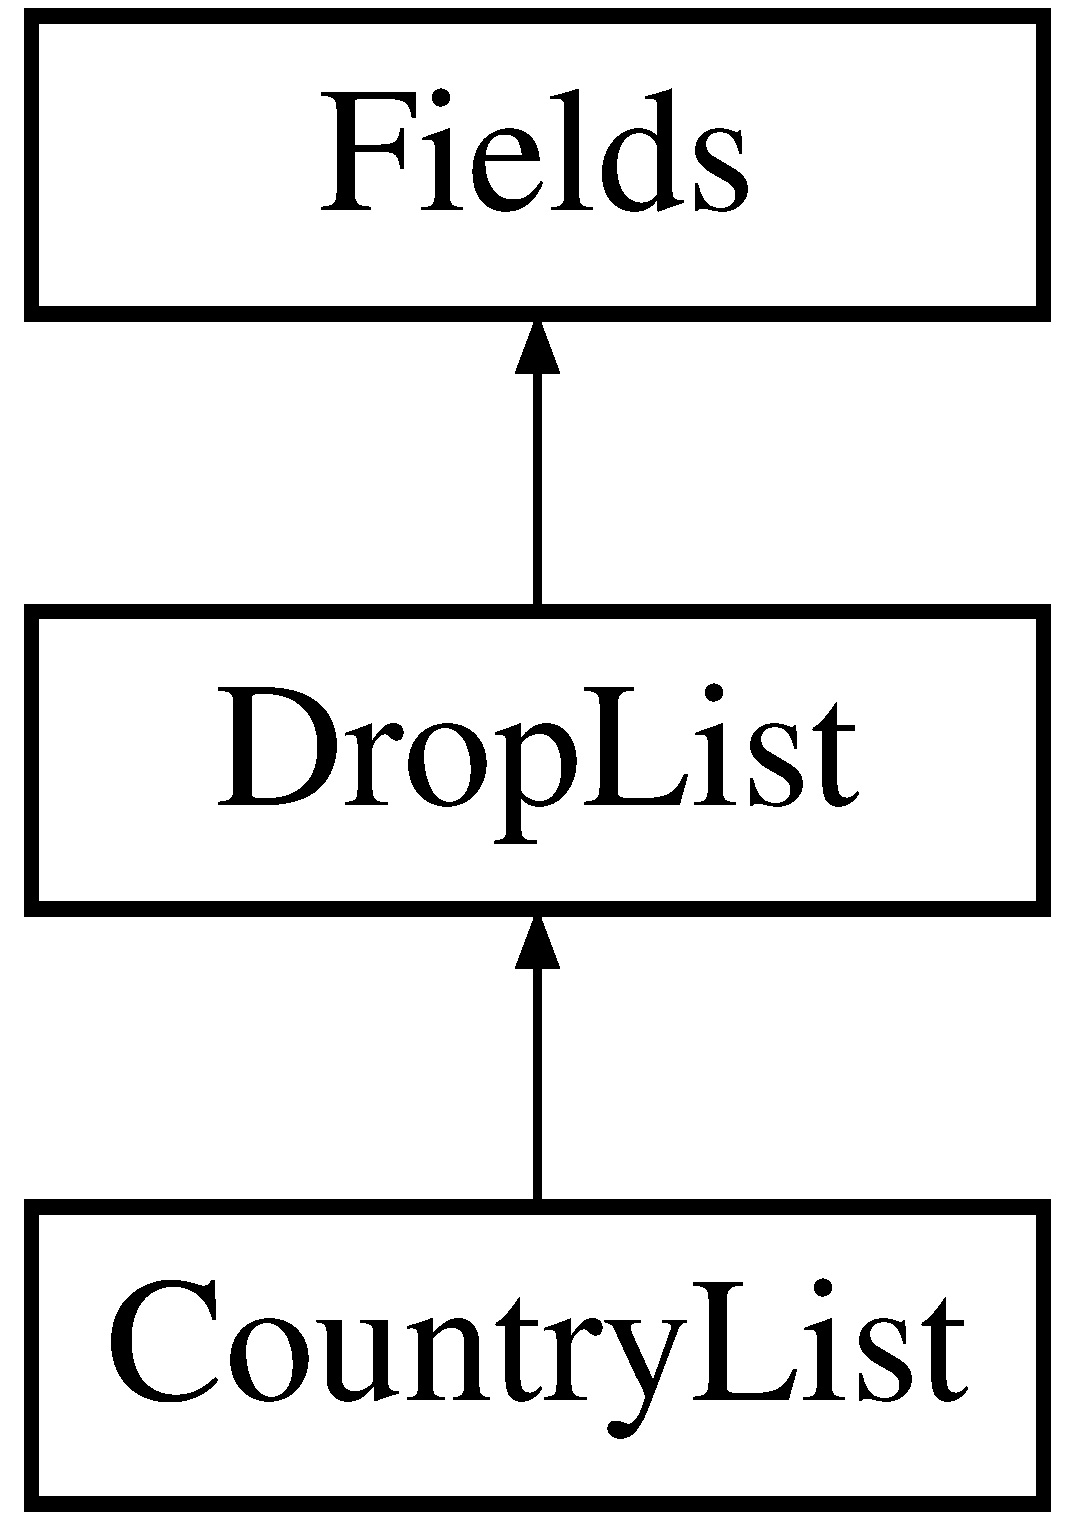
\includegraphics[height=3.000000cm]{class_drop_list}
\end{center}
\end{figure}
\subsection*{Public Member Functions}
\begin{DoxyCompactItemize}
\item 
\hyperlink{class_drop_list_ae820b56637ba8a8d0c4de37d4313231a}{add\-Option} (\$key, \$value)
\begin{DoxyCompactList}\small\item\em Add options to \hyperlink{class_drop_list}{Drop\-List} field. \end{DoxyCompactList}\item 
\hypertarget{class_drop_list_a3c65f396966df9520cc32aceecdac142}{\hyperlink{class_drop_list_a3c65f396966df9520cc32aceecdac142}{delete\-Option} (\$key)}\label{class_drop_list_a3c65f396966df9520cc32aceecdac142}

\begin{DoxyCompactList}\small\item\em Delete an option based on it's key (html name) not value. \end{DoxyCompactList}\item 
\hypertarget{class_drop_list_a14814e04b348120748912692645f3a75}{\hyperlink{class_drop_list_a14814e04b348120748912692645f3a75}{get\-Contents} ()}\label{class_drop_list_a14814e04b348120748912692645f3a75}

\begin{DoxyCompactList}\small\item\em Get the value of the field as html format. Used by form. \end{DoxyCompactList}\item 
\hypertarget{class_drop_list_adc30a2a4d3e48cb6aee21562afbc4022}{{\bfseries get\-Default} ()}\label{class_drop_list_adc30a2a4d3e48cb6aee21562afbc4022}

\item 
\hypertarget{class_drop_list_a04fffd28e332264bc38d2d07332a0db3}{{\bfseries set\-Default} (\$option)}\label{class_drop_list_a04fffd28e332264bc38d2d07332a0db3}

\end{DoxyCompactItemize}
\subsection*{Additional Inherited Members}


\subsection{Detailed Description}
Drop list field for \hyperlink{class_form}{Form} Used for drop down lists within html form. 

\subsection{Member Function Documentation}
\hypertarget{class_drop_list_ae820b56637ba8a8d0c4de37d4313231a}{\index{Drop\-List@{Drop\-List}!add\-Option@{add\-Option}}
\index{add\-Option@{add\-Option}!DropList@{Drop\-List}}
\subsubsection[{add\-Option}]{\setlength{\rightskip}{0pt plus 5cm}add\-Option (
\begin{DoxyParamCaption}
\item[{}]{\$key, }
\item[{}]{\$value}
\end{DoxyParamCaption}
)}}\label{class_drop_list_ae820b56637ba8a8d0c4de37d4313231a}


Add options to \hyperlink{class_drop_list}{Drop\-List} field. 

\$key is html name of the option and \$value is the physical value data of the option. 

The documentation for this class was generated from the following file\-:\begin{DoxyCompactItemize}
\item 
Form.\-php\end{DoxyCompactItemize}

\hypertarget{class_fields}{\section{Fields Class Reference}
\label{class_fields}\index{Fields@{Fields}}
}


Abstract class for fields.  


Inheritance diagram for Fields\-:\begin{figure}[H]
\begin{center}
\leavevmode
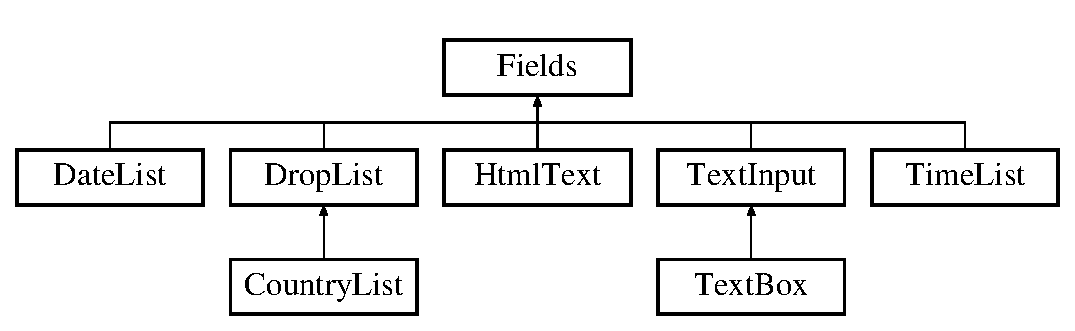
\includegraphics[height=3.000000cm]{class_fields}
\end{center}
\end{figure}
\subsection*{Public Member Functions}
\begin{DoxyCompactItemize}
\item 
\hyperlink{class_fields_ac610fc08cbb0781b26136636de129bc0}{\-\_\-\-\_\-construct} (\$nm)
\begin{DoxyCompactList}\small\item\em Default constructor for field. \end{DoxyCompactList}\item 
\hypertarget{class_fields_a421831a265621325e1fdd19aace0c758}{\hyperlink{class_fields_a421831a265621325e1fdd19aace0c758}{\-\_\-\-\_\-destruct} ()}\label{class_fields_a421831a265621325e1fdd19aace0c758}

\begin{DoxyCompactList}\small\item\em Default de-\/constructor for class. \end{DoxyCompactList}\item 
\hypertarget{class_fields_a14814e04b348120748912692645f3a75}{\hyperlink{class_fields_a14814e04b348120748912692645f3a75}{get\-Contents} ()}\label{class_fields_a14814e04b348120748912692645f3a75}

\begin{DoxyCompactList}\small\item\em Get the value of the field as html format. Used by form. Must be overridden. \end{DoxyCompactList}\item 
\hypertarget{class_fields_a12c89cd171dcdb78019486e439cbc167}{\hyperlink{class_fields_a12c89cd171dcdb78019486e439cbc167}{get\-Has\-Break} ()}\label{class_fields_a12c89cd171dcdb78019486e439cbc167}

\begin{DoxyCompactList}\small\item\em Get if there should be a break after the field. \end{DoxyCompactList}\item 
\hypertarget{class_fields_ad299af8d6a2adbe4e29c512e97820887}{\hyperlink{class_fields_ad299af8d6a2adbe4e29c512e97820887}{set\-Has\-Break} (\$nm)}\label{class_fields_ad299af8d6a2adbe4e29c512e97820887}

\begin{DoxyCompactList}\small\item\em Set if there should be a break after the field. \end{DoxyCompactList}\item 
\hyperlink{class_fields_af349b62dcfca9af90e20bd0b2766ce5e}{set\-Shown\-Name} (\$nm)
\begin{DoxyCompactList}\small\item\em Set label value, or displayed name before the field. \end{DoxyCompactList}\item 
\hyperlink{class_fields_aa377fa79244ee3146a650fcff9d709e4}{get\-Shown\-Name} ()
\begin{DoxyCompactList}\small\item\em Get label value, or displayed name before the field. \end{DoxyCompactList}\item 
\hypertarget{class_fields_a765e454543169586ea855cde5dd64129}{\hyperlink{class_fields_a765e454543169586ea855cde5dd64129}{get\-Has\-Div} ()}\label{class_fields_a765e454543169586ea855cde5dd64129}

\begin{DoxyCompactList}\small\item\em Get if field is wrapped in div. \end{DoxyCompactList}\item 
\hypertarget{class_fields_a7cf09e8ea450f02764ad51475f5eccf3}{\hyperlink{class_fields_a7cf09e8ea450f02764ad51475f5eccf3}{set\-Has\-Div} (\$nm)}\label{class_fields_a7cf09e8ea450f02764ad51475f5eccf3}

\begin{DoxyCompactList}\small\item\em Set if field is wrapped in div. \end{DoxyCompactList}\item 
\hyperlink{class_fields_a013b668cd0771a560d9f8dd061badb82}{set\-Overide\-Def} (\$overide)
\begin{DoxyCompactList}\small\item\em Give a function with string return for override default \hyperlink{class_fields_a14814e04b348120748912692645f3a75}{Fields\-::get\-Contents()}. \end{DoxyCompactList}\item 
\hypertarget{class_fields_a0698530a58faba482d4d427815d7d2af}{\hyperlink{class_fields_a0698530a58faba482d4d427815d7d2af}{get\-Overide\-Def} ()}\label{class_fields_a0698530a58faba482d4d427815d7d2af}

\begin{DoxyCompactList}\small\item\em Returns an override function if it exists. Else returns empty. \end{DoxyCompactList}\item 
\hypertarget{class_fields_aaf2bb7deba74bb0f994044954bd74ff3}{\hyperlink{class_fields_aaf2bb7deba74bb0f994044954bd74ff3}{set\-Default} (\$d)}\label{class_fields_aaf2bb7deba74bb0f994044954bd74ff3}

\begin{DoxyCompactList}\small\item\em Set html value of the field. \end{DoxyCompactList}\item 
\hypertarget{class_fields_adc30a2a4d3e48cb6aee21562afbc4022}{\hyperlink{class_fields_adc30a2a4d3e48cb6aee21562afbc4022}{get\-Default} ()}\label{class_fields_adc30a2a4d3e48cb6aee21562afbc4022}

\begin{DoxyCompactList}\small\item\em Get html value of the field. \end{DoxyCompactList}\item 
\hypertarget{class_fields_a3d0963e68bb313b163a73f2803c64600}{\hyperlink{class_fields_a3d0963e68bb313b163a73f2803c64600}{get\-Name} ()}\label{class_fields_a3d0963e68bb313b163a73f2803c64600}

\begin{DoxyCompactList}\small\item\em Get unique html name of the field. \end{DoxyCompactList}\item 
\hyperlink{class_fields_a6f75ffe7d98c9e375394d63f8d379b2d}{set\-Class} (\$nm)
\begin{DoxyCompactList}\small\item\em Set custom field class. \end{DoxyCompactList}\item 
\hyperlink{class_fields_a23ecbde357f7f6bde5a50f876334a74d}{get\-Class} ()
\begin{DoxyCompactList}\small\item\em Get custom field class. \end{DoxyCompactList}\item 
\hyperlink{class_fields_a4e25c00802ca9e9afb52a9177014fea7}{set\-Div\-Class} (\$nm)
\begin{DoxyCompactList}\small\item\em Set custom div classes, can be multiple. \end{DoxyCompactList}\item 
\hypertarget{class_fields_aeb623d3ef75a148185d6e14f7369f452}{\hyperlink{class_fields_aeb623d3ef75a148185d6e14f7369f452}{get\-Div\-Class} ()}\label{class_fields_aeb623d3ef75a148185d6e14f7369f452}

\begin{DoxyCompactList}\small\item\em Get custom div classes for field. \end{DoxyCompactList}\item 
\hypertarget{class_fields_ad8196fba0b5aa1f325ab4b46477bf147}{\hyperlink{class_fields_ad8196fba0b5aa1f325ab4b46477bf147}{set\-Finalization} (\$dn)}\label{class_fields_ad8196fba0b5aa1f325ab4b46477bf147}

\begin{DoxyCompactList}\small\item\em May be deprecated\-: Used for specific task from previous client. \end{DoxyCompactList}\item 
\hypertarget{class_fields_a971544d42becf229e8b472fc4bd6662c}{\hyperlink{class_fields_a971544d42becf229e8b472fc4bd6662c}{get\-Finalization} ()}\label{class_fields_a971544d42becf229e8b472fc4bd6662c}

\begin{DoxyCompactList}\small\item\em May be deprecated\-: Used for specific task from previous client. \end{DoxyCompactList}\item 
\hypertarget{class_fields_aa72ae1ae3cc8dd09eccc5d0db3c1b57e}{\hyperlink{class_fields_aa72ae1ae3cc8dd09eccc5d0db3c1b57e}{set\-Will\-Display\-Name} (\$dn)}\label{class_fields_aa72ae1ae3cc8dd09eccc5d0db3c1b57e}

\begin{DoxyCompactList}\small\item\em Set whether or not a label will appear before the actual field. \end{DoxyCompactList}\item 
\hypertarget{class_fields_a5079e029359e2c1d8a16e6041fcea9e1}{\hyperlink{class_fields_a5079e029359e2c1d8a16e6041fcea9e1}{get\-Will\-Display\-Name} ()}\label{class_fields_a5079e029359e2c1d8a16e6041fcea9e1}

\begin{DoxyCompactList}\small\item\em Get whether or not a label will appear before the actual field. \end{DoxyCompactList}\item 
\hypertarget{class_fields_a0a13d142a737f59d9b56857a937212aa}{\hyperlink{class_fields_a0a13d142a737f59d9b56857a937212aa}{set\-Is\-Capital} (\$bool)}\label{class_fields_a0a13d142a737f59d9b56857a937212aa}

\begin{DoxyCompactList}\small\item\em Set whether or not to capitalize for the letter of the field. \end{DoxyCompactList}\item 
\hypertarget{class_fields_ac52f815397270d01eeef3a2d33ce05cf}{\hyperlink{class_fields_ac52f815397270d01eeef3a2d33ce05cf}{get\-Is\-Capital} ()}\label{class_fields_ac52f815397270d01eeef3a2d33ce05cf}

\begin{DoxyCompactList}\small\item\em Get whether or not to capitalize for the first letter of the field. \end{DoxyCompactList}\end{DoxyCompactItemize}
\subsection*{Protected Attributes}
\begin{DoxyCompactItemize}
\item 
\hypertarget{class_fields_a6efc15b5a2314dd4b5aaa556a375c6d6}{{\bfseries \$data}}\label{class_fields_a6efc15b5a2314dd4b5aaa556a375c6d6}

\item 
\hypertarget{class_fields_a9f8f890e2d5fb4b002a11db42621b997}{{\bfseries \$def}}\label{class_fields_a9f8f890e2d5fb4b002a11db42621b997}

\item 
\hypertarget{class_fields_ab2fc40d43824ea3e1ce5d86dee0d763b}{{\bfseries \$name}}\label{class_fields_ab2fc40d43824ea3e1ce5d86dee0d763b}

\item 
\hypertarget{class_fields_a7c698bda11f44f45e6a5fd82e1ddc01e}{{\bfseries \$shown\-Name}}\label{class_fields_a7c698bda11f44f45e6a5fd82e1ddc01e}

\item 
\hypertarget{class_fields_ac1b12cd5f2bbc3d7dcff91e4e27dfee6}{{\bfseries \$display\-Name}}\label{class_fields_ac1b12cd5f2bbc3d7dcff91e4e27dfee6}

\item 
\hypertarget{class_fields_aa84bd2be5a4f81cade0930c6694a26fa}{{\bfseries \$has\-Break}}\label{class_fields_aa84bd2be5a4f81cade0930c6694a26fa}

\item 
\hypertarget{class_fields_ad2991a33c97b365c8b41fa1f644bb01a}{{\bfseries \$show\-Finalization}}\label{class_fields_ad2991a33c97b365c8b41fa1f644bb01a}

\item 
\hypertarget{class_fields_a266ed9d0a8228a3912e3a9ee946e76e3}{{\bfseries \$is\-Capital}}\label{class_fields_a266ed9d0a8228a3912e3a9ee946e76e3}

\item 
\hypertarget{class_fields_ae7e3ab624061054c47a97d31a4a0198f}{{\bfseries \$class\-Val}}\label{class_fields_ae7e3ab624061054c47a97d31a4a0198f}

\item 
\hypertarget{class_fields_a6085e95306e812d296babfcb8b1abbce}{{\bfseries \$div\-Class\-Val}}\label{class_fields_a6085e95306e812d296babfcb8b1abbce}

\item 
\hypertarget{class_fields_a124a98018a4d5ac1355db06c8f0d754f}{{\bfseries \$overide\-Func}}\label{class_fields_a124a98018a4d5ac1355db06c8f0d754f}

\item 
\hypertarget{class_fields_af159a07f440f1e110d9852e0127efe0e}{{\bfseries \$has\-Div}}\label{class_fields_af159a07f440f1e110d9852e0127efe0e}

\end{DoxyCompactItemize}


\subsection{Detailed Description}
Abstract class for fields. 

Has basic field properties. All fields that are used in form must extend this class. 

\subsection{Constructor \& Destructor Documentation}
\hypertarget{class_fields_ac610fc08cbb0781b26136636de129bc0}{\index{Fields@{Fields}!\-\_\-\-\_\-construct@{\-\_\-\-\_\-construct}}
\index{\-\_\-\-\_\-construct@{\-\_\-\-\_\-construct}!Fields@{Fields}}
\subsubsection[{\-\_\-\-\_\-construct}]{\setlength{\rightskip}{0pt plus 5cm}\-\_\-\-\_\-construct (
\begin{DoxyParamCaption}
\item[{}]{\$nm}
\end{DoxyParamCaption}
)}}\label{class_fields_ac610fc08cbb0781b26136636de129bc0}


Default constructor for field. 

Requires a name for the field. Name used for both display and html names. Display name can then be over written by \hyperlink{class_fields_af349b62dcfca9af90e20bd0b2766ce5e}{Fields\-::set\-Shown\-Name}(\$nm). 

\subsection{Member Function Documentation}
\hypertarget{class_fields_a23ecbde357f7f6bde5a50f876334a74d}{\index{Fields@{Fields}!get\-Class@{get\-Class}}
\index{get\-Class@{get\-Class}!Fields@{Fields}}
\subsubsection[{get\-Class}]{\setlength{\rightskip}{0pt plus 5cm}get\-Class (
\begin{DoxyParamCaption}
{}
\end{DoxyParamCaption}
)}}\label{class_fields_a23ecbde357f7f6bde5a50f876334a74d}


Get custom field class. 

Gets custom field's html class only. Not the field's div class. Refer to \hyperlink{class_fields_aeb623d3ef75a148185d6e14f7369f452}{Fields\-::get\-Div\-Class()} \hypertarget{class_fields_aa377fa79244ee3146a650fcff9d709e4}{\index{Fields@{Fields}!get\-Shown\-Name@{get\-Shown\-Name}}
\index{get\-Shown\-Name@{get\-Shown\-Name}!Fields@{Fields}}
\subsubsection[{get\-Shown\-Name}]{\setlength{\rightskip}{0pt plus 5cm}get\-Shown\-Name (
\begin{DoxyParamCaption}
{}
\end{DoxyParamCaption}
)}}\label{class_fields_aa377fa79244ee3146a650fcff9d709e4}


Get label value, or displayed name before the field. 

Does not affect the html attribute name of the field. Only changes the name displayed in web page. \hyperlink{class_fields_a5079e029359e2c1d8a16e6041fcea9e1}{Fields\-::get\-Will\-Display\-Name()} must be true in order for name to appear. \hypertarget{class_fields_a6f75ffe7d98c9e375394d63f8d379b2d}{\index{Fields@{Fields}!set\-Class@{set\-Class}}
\index{set\-Class@{set\-Class}!Fields@{Fields}}
\subsubsection[{set\-Class}]{\setlength{\rightskip}{0pt plus 5cm}set\-Class (
\begin{DoxyParamCaption}
\item[{}]{\$nm}
\end{DoxyParamCaption}
)}}\label{class_fields_a6f75ffe7d98c9e375394d63f8d379b2d}


Set custom field class. 

Sets custom field's html class only. Not the field's div class. Refer to \hyperlink{class_fields_a4e25c00802ca9e9afb52a9177014fea7}{Fields\-::set\-Div\-Class}(\$nm) \hypertarget{class_fields_a4e25c00802ca9e9afb52a9177014fea7}{\index{Fields@{Fields}!set\-Div\-Class@{set\-Div\-Class}}
\index{set\-Div\-Class@{set\-Div\-Class}!Fields@{Fields}}
\subsubsection[{set\-Div\-Class}]{\setlength{\rightskip}{0pt plus 5cm}set\-Div\-Class (
\begin{DoxyParamCaption}
\item[{}]{\$nm}
\end{DoxyParamCaption}
)}}\label{class_fields_a4e25c00802ca9e9afb52a9177014fea7}


Set custom div classes, can be multiple. 

Show div must be true for this function to work properly. Check with \hyperlink{class_fields_a765e454543169586ea855cde5dd64129}{Fields\-::get\-Has\-Div()} and use \hyperlink{class_fields_a7cf09e8ea450f02764ad51475f5eccf3}{Fields\-::set\-Has\-Div}(\$nm) to set. Does not refer to field's html class only it's div. Refer to Field\-::set\-Class(\$nm). \hypertarget{class_fields_a013b668cd0771a560d9f8dd061badb82}{\index{Fields@{Fields}!set\-Overide\-Def@{set\-Overide\-Def}}
\index{set\-Overide\-Def@{set\-Overide\-Def}!Fields@{Fields}}
\subsubsection[{set\-Overide\-Def}]{\setlength{\rightskip}{0pt plus 5cm}set\-Overide\-Def (
\begin{DoxyParamCaption}
\item[{}]{\$overide}
\end{DoxyParamCaption}
)}}\label{class_fields_a013b668cd0771a560d9f8dd061badb82}


Give a function with string return for override default \hyperlink{class_fields_a14814e04b348120748912692645f3a75}{Fields\-::get\-Contents()}. 

The given function will run and edit the value returned in \hyperlink{class_form_af9462fe23a23d3339788f006ed4553e5}{Form\-::get\-Array\-Value()} instead of just the usual \hyperlink{class_fields_a14814e04b348120748912692645f3a75}{Fields\-::get\-Contents()} when \hyperlink{class_form}{Form} parses the this field. Please note that the function must have the following parameters\-: one parameter for default value of field (dependent on field) and one parameter for an array of fields (the \hyperlink{class_form_af9462fe23a23d3339788f006ed4553e5}{Form\-::get\-Array\-Value()} arrays except with \hyperlink{class_html_text}{Html\-Text} fields). Function must also return a string value to overide the value of the field. Please note that this is a very dangerous function use with caution. Mainly used for custom values in locked input fields. \hypertarget{class_fields_af349b62dcfca9af90e20bd0b2766ce5e}{\index{Fields@{Fields}!set\-Shown\-Name@{set\-Shown\-Name}}
\index{set\-Shown\-Name@{set\-Shown\-Name}!Fields@{Fields}}
\subsubsection[{set\-Shown\-Name}]{\setlength{\rightskip}{0pt plus 5cm}set\-Shown\-Name (
\begin{DoxyParamCaption}
\item[{}]{\$nm}
\end{DoxyParamCaption}
)}}\label{class_fields_af349b62dcfca9af90e20bd0b2766ce5e}


Set label value, or displayed name before the field. 

Does not affect the html attribute name of the field. Only changes the name displayed in web page. \hyperlink{class_fields_a5079e029359e2c1d8a16e6041fcea9e1}{Fields\-::get\-Will\-Display\-Name()} must be true in order for name to appear. 

The documentation for this class was generated from the following file\-:\begin{DoxyCompactItemize}
\item 
Form.\-php\end{DoxyCompactItemize}

\hypertarget{class_form}{\section{Form Class Reference}
\label{class_form}\index{Form@{Form}}
}


A canvas for form field (components), form info, and display info.  


\subsection*{Public Member Functions}
\begin{DoxyCompactItemize}
\item 
\hyperlink{class_form_af40041b2b1c6558837ba8596fe8e0552}{\-\_\-\-\_\-construct} (\$datauser, \$database, \$table)
\begin{DoxyCompactList}\small\item\em Constructor for \hyperlink{class_form}{Form} class. \end{DoxyCompactList}\item 
\hyperlink{class_form_a421831a265621325e1fdd19aace0c758}{\-\_\-\-\_\-destruct} ()
\item 
\hyperlink{class_form_a1fdf528a1c08761a1cd21deeac02655a}{add\-Field} (\$fobject)
\begin{DoxyCompactList}\small\item\em Add a new field to the From. \end{DoxyCompactList}\item 
\hyperlink{class_form_aff667c8e7e2da76ea9ba77bc12f20027}{get\-Fields} ()
\begin{DoxyCompactList}\small\item\em Gets an array of \hyperlink{class_fields}{Fields} within \hyperlink{class_form}{Form}. \end{DoxyCompactList}\item 
\hyperlink{class_form_a78d90edb0ba539b78fdd44a7c7f9bfac}{add\-H\-T\-M\-L\-Text} (\$text)
\begin{DoxyCompactList}\small\item\em May be deprecated\-: Adds H\-T\-M\-L to form, uses html field. \end{DoxyCompactList}\item 
\hyperlink{class_form_a9a5e9a31d4ef1eb8bdda31189c9ba63f}{set\-Button\-Value} (\$button)
\begin{DoxyCompactList}\small\item\em Set display button string value/text. \end{DoxyCompactList}\item 
\hyperlink{class_form_ac49688299ee6efe70a6a4c6ef3e36e2d}{get\-Button\-Value} ()
\begin{DoxyCompactList}\small\item\em Get value/display text of the button. \end{DoxyCompactList}\item 
\hyperlink{class_form_a533a47491c1ff122561ffcd310287c60}{set\-Button\-Name} (\$name)
\begin{DoxyCompactList}\small\item\em Set button value for html. \end{DoxyCompactList}\item 
\hyperlink{class_form_a2188941ec159bfb3f902dfc5583373aa}{get\-Button\-Name} ()
\begin{DoxyCompactList}\small\item\em Get name of the button. \end{DoxyCompactList}\item 
\hyperlink{class_form_a19b9c02f0d7cb966dc089c9bf360ba9a}{get\-Value} (\$nm)
\begin{DoxyCompactList}\small\item\em Get the field's default value stored in form based on the name of the component. \end{DoxyCompactList}\item 
\hyperlink{class_form_a49dd73fe22e8f5cc54c4a8c5d860288a}{set\-Value} (\$nm, \$val)
\begin{DoxyCompactList}\small\item\em Set default value for a field in form. \end{DoxyCompactList}\item 
\hyperlink{class_form_a0fc192b82e0cc5ddfeb120046d3fff36}{set\-Array\-Value} (\$post)
\begin{DoxyCompactList}\small\item\em Set default value for field in form based on array. \end{DoxyCompactList}\item 
\hyperlink{class_form_af9462fe23a23d3339788f006ed4553e5}{get\-Array\-Value} ()
\begin{DoxyCompactList}\small\item\em Get all the field's default value in form as an array. \end{DoxyCompactList}\item 
\hypertarget{class_form_a8b1e7e0b28b4e5495060b1119fd2d539}{\hyperlink{class_form_a8b1e7e0b28b4e5495060b1119fd2d539}{set\-Database} (\$database)}\label{class_form_a8b1e7e0b28b4e5495060b1119fd2d539}

\begin{DoxyCompactList}\small\item\em Set S\-Q\-L database name for \hyperlink{class_form}{Form}. \end{DoxyCompactList}\item 
\hypertarget{class_form_a728138a9219e8751278542c3a8c5e3a9}{\hyperlink{class_form_a728138a9219e8751278542c3a8c5e3a9}{get\-Database} ()}\label{class_form_a728138a9219e8751278542c3a8c5e3a9}

\begin{DoxyCompactList}\small\item\em Get S\-Q\-L database name for \hyperlink{class_form}{Form}. \end{DoxyCompactList}\item 
\hypertarget{class_form_aa826f100dc28f64afa9687013de95a4e}{\hyperlink{class_form_aa826f100dc28f64afa9687013de95a4e}{set\-Data\-User} (\$datauser)}\label{class_form_aa826f100dc28f64afa9687013de95a4e}

\begin{DoxyCompactList}\small\item\em Set S\-Q\-L user for \hyperlink{class_form}{Form}. \end{DoxyCompactList}\item 
\hypertarget{class_form_a31b30bf9e93dae44203a91f17a0314ef}{\hyperlink{class_form_a31b30bf9e93dae44203a91f17a0314ef}{get\-Data\-User} ()}\label{class_form_a31b30bf9e93dae44203a91f17a0314ef}

\begin{DoxyCompactList}\small\item\em Get S\-Q\-L user for \hyperlink{class_form}{Form}. \end{DoxyCompactList}\item 
\hypertarget{class_form_aa845c297fed99536c5c6768a469ddfb7}{\hyperlink{class_form_aa845c297fed99536c5c6768a469ddfb7}{set\-Table} (\$table)}\label{class_form_aa845c297fed99536c5c6768a469ddfb7}

\begin{DoxyCompactList}\small\item\em Set S\-Q\-L table for \hyperlink{class_form}{Form}. \end{DoxyCompactList}\item 
\hypertarget{class_form_aa0dd4bf57d57bc2a3697e40c9f6bddce}{\hyperlink{class_form_aa0dd4bf57d57bc2a3697e40c9f6bddce}{get\-Table} ()}\label{class_form_aa0dd4bf57d57bc2a3697e40c9f6bddce}

\begin{DoxyCompactList}\small\item\em Get S\-Q\-L table for \hyperlink{class_form}{Form}. \end{DoxyCompactList}\item 
\hyperlink{class_form_a78b6c3cfdb107a1703e33e8cbdbe325a}{set\-Id\-Value} (\$id\-Value)
\begin{DoxyCompactList}\small\item\em Set S\-Q\-L Id value for \hyperlink{class_form}{Form}. \end{DoxyCompactList}\item 
\hyperlink{class_form_ac07b8eeb46c3b8153ce94196498d7d4f}{get\-Id\-Value} ()
\begin{DoxyCompactList}\small\item\em Get S\-Q\-L Id variable value. \end{DoxyCompactList}\item 
\hyperlink{class_form_a87313ad678fb2a2a8efb435cf0bdb9a0}{set\-Id} (\$id)
\begin{DoxyCompactList}\small\item\em Set S\-Q\-L Id variable name. \end{DoxyCompactList}\item 
\hyperlink{class_form_a12251d0c022e9e21c137a105ff683f13}{get\-Id} ()
\begin{DoxyCompactList}\small\item\em Get S\-Q\-L Id variable name. \end{DoxyCompactList}\item 
\hyperlink{class_form_a6d1d275ab79fc98419e621981e53ed0a}{delete\-Field} (\$nm)
\begin{DoxyCompactList}\small\item\em Delete a field in form. \end{DoxyCompactList}\item 
\hyperlink{class_form_a6aed11d79758a2d06062c8cd94bab221}{get\-Form} ()
\begin{DoxyCompactList}\small\item\em Get display contents for form. \end{DoxyCompactList}\item 
\hyperlink{class_form_a1ad69c3a61165fa41d9224d4f5a6de1c}{set\-Form\-Name} (\$nm)
\begin{DoxyCompactList}\small\item\em Set the form name. \end{DoxyCompactList}\end{DoxyCompactItemize}
\subsection*{Private Attributes}
\begin{DoxyCompactItemize}
\item 
\hypertarget{class_form_a83e4d6721f3491a4fd780dbd3ce1a3c0}{\hyperlink{class_form_a83e4d6721f3491a4fd780dbd3ce1a3c0}{\$field}}\label{class_form_a83e4d6721f3491a4fd780dbd3ce1a3c0}

\begin{DoxyCompactList}\small\item\em Array to hold fields. \end{DoxyCompactList}\item 
\hypertarget{class_form_aeb04f2cbd555f3a0791905851b4d27e1}{\hyperlink{class_form_aeb04f2cbd555f3a0791905851b4d27e1}{\$formname}}\label{class_form_aeb04f2cbd555f3a0791905851b4d27e1}

\begin{DoxyCompactList}\small\item\em String to hold form name, used for form class. Default to 'form'. \end{DoxyCompactList}\item 
\hypertarget{class_form_a660aa7e36590fa523b680c24fc0c90bb}{\hyperlink{class_form_a660aa7e36590fa523b680c24fc0c90bb}{\$datauser}}\label{class_form_a660aa7e36590fa523b680c24fc0c90bb}

\begin{DoxyCompactList}\small\item\em S\-Q\-L user name. \end{DoxyCompactList}\item 
\hypertarget{class_form_a7691c0162d89de0b6ba47edcd8ba8878}{\hyperlink{class_form_a7691c0162d89de0b6ba47edcd8ba8878}{\$database}}\label{class_form_a7691c0162d89de0b6ba47edcd8ba8878}

\begin{DoxyCompactList}\small\item\em S\-Q\-L database name. \end{DoxyCompactList}\item 
\hypertarget{class_form_ae8876a14058f368335baccf35af4a22b}{\hyperlink{class_form_ae8876a14058f368335baccf35af4a22b}{\$table}}\label{class_form_ae8876a14058f368335baccf35af4a22b}

\begin{DoxyCompactList}\small\item\em S\-Q\-L table name. \end{DoxyCompactList}\item 
\hypertarget{class_form_ae97941710d863131c700f069b109991e}{\hyperlink{class_form_ae97941710d863131c700f069b109991e}{\$id}}\label{class_form_ae97941710d863131c700f069b109991e}

\begin{DoxyCompactList}\small\item\em S\-Q\-L unique id name, default to 'usr'. \end{DoxyCompactList}\item 
\hypertarget{class_form_a49e4e8fba70a36c568c8ee2505ba914a}{\hyperlink{class_form_a49e4e8fba70a36c568c8ee2505ba914a}{\$id\-Value}}\label{class_form_a49e4e8fba70a36c568c8ee2505ba914a}

\begin{DoxyCompactList}\small\item\em S\-Q\-L unique id value, default to 'Master'. \end{DoxyCompactList}\item 
\hypertarget{class_form_a023f71dca77d38c658f9be1e32f3f09a}{\hyperlink{class_form_a023f71dca77d38c658f9be1e32f3f09a}{\$button\-Value}}\label{class_form_a023f71dca77d38c658f9be1e32f3f09a}

\begin{DoxyCompactList}\small\item\em Holds form button value/display text. \end{DoxyCompactList}\item 
\hypertarget{class_form_a6e20c1bfd57561f7501fc132a9eaab5f}{\hyperlink{class_form_a6e20c1bfd57561f7501fc132a9eaab5f}{\$button\-Name}}\label{class_form_a6e20c1bfd57561f7501fc132a9eaab5f}

\begin{DoxyCompactList}\small\item\em Holds form button class name. \end{DoxyCompactList}\end{DoxyCompactItemize}


\subsection{Detailed Description}
A canvas for form field (components), form info, and display info. 

Manages each component in an array. Stores attributes to form. Does not contain display info, each individual component does. 

\subsection{Constructor \& Destructor Documentation}
\hypertarget{class_form_af40041b2b1c6558837ba8596fe8e0552}{\index{Form@{Form}!\-\_\-\-\_\-construct@{\-\_\-\-\_\-construct}}
\index{\-\_\-\-\_\-construct@{\-\_\-\-\_\-construct}!Form@{Form}}
\subsubsection[{\-\_\-\-\_\-construct}]{\setlength{\rightskip}{0pt plus 5cm}\-\_\-\-\_\-construct (
\begin{DoxyParamCaption}
\item[{}]{\$datauser, }
\item[{}]{\$database, }
\item[{}]{\$table}
\end{DoxyParamCaption}
)}}\label{class_form_af40041b2b1c6558837ba8596fe8e0552}


Constructor for \hyperlink{class_form}{Form} class. 

Requires a user, database, and table for S\-Q\-L use in \hyperlink{class_form}{Form}. This decision was made as forms must have some sort of association with S\-Q\-L. May be changed if not heavily used. \hypertarget{class_form_a421831a265621325e1fdd19aace0c758}{\index{Form@{Form}!\-\_\-\-\_\-destruct@{\-\_\-\-\_\-destruct}}
\index{\-\_\-\-\_\-destruct@{\-\_\-\-\_\-destruct}!Form@{Form}}
\subsubsection[{\-\_\-\-\_\-destruct}]{\setlength{\rightskip}{0pt plus 5cm}\-\_\-\-\_\-destruct (
\begin{DoxyParamCaption}
{}
\end{DoxyParamCaption}
)}}\label{class_form_a421831a265621325e1fdd19aace0c758}
Unsets stored fields. 

\subsection{Member Function Documentation}
\hypertarget{class_form_a1fdf528a1c08761a1cd21deeac02655a}{\index{Form@{Form}!add\-Field@{add\-Field}}
\index{add\-Field@{add\-Field}!Form@{Form}}
\subsubsection[{add\-Field}]{\setlength{\rightskip}{0pt plus 5cm}add\-Field (
\begin{DoxyParamCaption}
\item[{}]{\$fobject}
\end{DoxyParamCaption}
)}}\label{class_form_a1fdf528a1c08761a1cd21deeac02655a}


Add a new field to the From. 

The html name of the field must be unique. Name is used for an unqiue key in form. \hypertarget{class_form_a78d90edb0ba539b78fdd44a7c7f9bfac}{\index{Form@{Form}!add\-H\-T\-M\-L\-Text@{add\-H\-T\-M\-L\-Text}}
\index{add\-H\-T\-M\-L\-Text@{add\-H\-T\-M\-L\-Text}!Form@{Form}}
\subsubsection[{add\-H\-T\-M\-L\-Text}]{\setlength{\rightskip}{0pt plus 5cm}add\-H\-T\-M\-L\-Text (
\begin{DoxyParamCaption}
\item[{}]{\$text}
\end{DoxyParamCaption}
)}}\label{class_form_a78d90edb0ba539b78fdd44a7c7f9bfac}


May be deprecated\-: Adds H\-T\-M\-L to form, uses html field. 

Adds H\-T\-M\-L directly into form without creating extra components. Used to be used for the early days of Alpha. Now is unnecessary due to component design decisions. \hypertarget{class_form_a6d1d275ab79fc98419e621981e53ed0a}{\index{Form@{Form}!delete\-Field@{delete\-Field}}
\index{delete\-Field@{delete\-Field}!Form@{Form}}
\subsubsection[{delete\-Field}]{\setlength{\rightskip}{0pt plus 5cm}delete\-Field (
\begin{DoxyParamCaption}
\item[{}]{\$nm}
\end{DoxyParamCaption}
)}}\label{class_form_a6d1d275ab79fc98419e621981e53ed0a}


Delete a field in form. 

Return true if field deleted successfully. False if field does not exist with given name. \hypertarget{class_form_af9462fe23a23d3339788f006ed4553e5}{\index{Form@{Form}!get\-Array\-Value@{get\-Array\-Value}}
\index{get\-Array\-Value@{get\-Array\-Value}!Form@{Form}}
\subsubsection[{get\-Array\-Value}]{\setlength{\rightskip}{0pt plus 5cm}get\-Array\-Value (
\begin{DoxyParamCaption}
{}
\end{DoxyParamCaption}
)}}\label{class_form_af9462fe23a23d3339788f006ed4553e5}


Get all the field's default value in form as an array. 

The key for the returned array is the unique html name from the fields. All values, except \hyperlink{class_html_text}{Html\-Text} is returned. \hypertarget{class_form_a2188941ec159bfb3f902dfc5583373aa}{\index{Form@{Form}!get\-Button\-Name@{get\-Button\-Name}}
\index{get\-Button\-Name@{get\-Button\-Name}!Form@{Form}}
\subsubsection[{get\-Button\-Name}]{\setlength{\rightskip}{0pt plus 5cm}get\-Button\-Name (
\begin{DoxyParamCaption}
{}
\end{DoxyParamCaption}
)}}\label{class_form_a2188941ec159bfb3f902dfc5583373aa}


Get name of the button. 

Note\-: Not the display text, but the name in html. \hypertarget{class_form_ac49688299ee6efe70a6a4c6ef3e36e2d}{\index{Form@{Form}!get\-Button\-Value@{get\-Button\-Value}}
\index{get\-Button\-Value@{get\-Button\-Value}!Form@{Form}}
\subsubsection[{get\-Button\-Value}]{\setlength{\rightskip}{0pt plus 5cm}get\-Button\-Value (
\begin{DoxyParamCaption}
{}
\end{DoxyParamCaption}
)}}\label{class_form_ac49688299ee6efe70a6a4c6ef3e36e2d}


Get value/display text of the button. 

Note\-: Not name attribute in html. It is the text displayed in the button. Refer to \hyperlink{class_form_ac49688299ee6efe70a6a4c6ef3e36e2d}{Form\-::get\-Button\-Value()}. \hypertarget{class_form_aff667c8e7e2da76ea9ba77bc12f20027}{\index{Form@{Form}!get\-Fields@{get\-Fields}}
\index{get\-Fields@{get\-Fields}!Form@{Form}}
\subsubsection[{get\-Fields}]{\setlength{\rightskip}{0pt plus 5cm}get\-Fields (
\begin{DoxyParamCaption}
{}
\end{DoxyParamCaption}
)}}\label{class_form_aff667c8e7e2da76ea9ba77bc12f20027}


Gets an array of \hyperlink{class_fields}{Fields} within \hyperlink{class_form}{Form}. 

Returns an array with key as \hyperlink{class_fields}{Fields} name and value as \hyperlink{class_fields}{Fields} class. \hypertarget{class_form_a6aed11d79758a2d06062c8cd94bab221}{\index{Form@{Form}!get\-Form@{get\-Form}}
\index{get\-Form@{get\-Form}!Form@{Form}}
\subsubsection[{get\-Form}]{\setlength{\rightskip}{0pt plus 5cm}get\-Form (
\begin{DoxyParamCaption}
{}
\end{DoxyParamCaption}
)}}\label{class_form_a6aed11d79758a2d06062c8cd94bab221}


Get display contents for form. 

Only returns display contents, does not display. Client must echo out the content returned. \hypertarget{class_form_a12251d0c022e9e21c137a105ff683f13}{\index{Form@{Form}!get\-Id@{get\-Id}}
\index{get\-Id@{get\-Id}!Form@{Form}}
\subsubsection[{get\-Id}]{\setlength{\rightskip}{0pt plus 5cm}get\-Id (
\begin{DoxyParamCaption}
{}
\end{DoxyParamCaption}
)}}\label{class_form_a12251d0c022e9e21c137a105ff683f13}


Get S\-Q\-L Id variable name. 

Gets the unique id variable name for S\-Q\-L. Not the value of the variable in S\-Q\-L. Refer to \hyperlink{class_form_ac07b8eeb46c3b8153ce94196498d7d4f}{Form\-::get\-Id\-Value()} for value. \hypertarget{class_form_ac07b8eeb46c3b8153ce94196498d7d4f}{\index{Form@{Form}!get\-Id\-Value@{get\-Id\-Value}}
\index{get\-Id\-Value@{get\-Id\-Value}!Form@{Form}}
\subsubsection[{get\-Id\-Value}]{\setlength{\rightskip}{0pt plus 5cm}get\-Id\-Value (
\begin{DoxyParamCaption}
{}
\end{DoxyParamCaption}
)}}\label{class_form_ac07b8eeb46c3b8153ce94196498d7d4f}


Get S\-Q\-L Id variable value. 

Gets the unique id variable value for S\-Q\-L. Not the name of the variable in S\-Q\-L. Refer to Form\-::get\-I\-D() for name. \hypertarget{class_form_a19b9c02f0d7cb966dc089c9bf360ba9a}{\index{Form@{Form}!get\-Value@{get\-Value}}
\index{get\-Value@{get\-Value}!Form@{Form}}
\subsubsection[{get\-Value}]{\setlength{\rightskip}{0pt plus 5cm}get\-Value (
\begin{DoxyParamCaption}
\item[{}]{\$nm}
\end{DoxyParamCaption}
)}}\label{class_form_a19b9c02f0d7cb966dc089c9bf360ba9a}


Get the field's default value stored in form based on the name of the component. 

The name of the form is created by the constructor of the component. Refer to\-: \hyperlink{class_fields_ac610fc08cbb0781b26136636de129bc0}{Fields\-::\-\_\-\-\_\-construct()}. \hypertarget{class_form_a0fc192b82e0cc5ddfeb120046d3fff36}{\index{Form@{Form}!set\-Array\-Value@{set\-Array\-Value}}
\index{set\-Array\-Value@{set\-Array\-Value}!Form@{Form}}
\subsubsection[{set\-Array\-Value}]{\setlength{\rightskip}{0pt plus 5cm}set\-Array\-Value (
\begin{DoxyParamCaption}
\item[{}]{\$post}
\end{DoxyParamCaption}
)}}\label{class_form_a0fc192b82e0cc5ddfeb120046d3fff36}


Set default value for field in form based on array. 

For single values, use Fields\-::set\-Value(\$nm, \$val). Array should have name of field as key and default value for field as value in array. \hypertarget{class_form_a533a47491c1ff122561ffcd310287c60}{\index{Form@{Form}!set\-Button\-Name@{set\-Button\-Name}}
\index{set\-Button\-Name@{set\-Button\-Name}!Form@{Form}}
\subsubsection[{set\-Button\-Name}]{\setlength{\rightskip}{0pt plus 5cm}set\-Button\-Name (
\begin{DoxyParamCaption}
\item[{}]{\$name}
\end{DoxyParamCaption}
)}}\label{class_form_a533a47491c1ff122561ffcd310287c60}


Set button value for html. 

Does not set the display text of the button. Modifies the name of button in html. Use this for css attributes. \hypertarget{class_form_a9a5e9a31d4ef1eb8bdda31189c9ba63f}{\index{Form@{Form}!set\-Button\-Value@{set\-Button\-Value}}
\index{set\-Button\-Value@{set\-Button\-Value}!Form@{Form}}
\subsubsection[{set\-Button\-Value}]{\setlength{\rightskip}{0pt plus 5cm}set\-Button\-Value (
\begin{DoxyParamCaption}
\item[{}]{\$button}
\end{DoxyParamCaption}
)}}\label{class_form_a9a5e9a31d4ef1eb8bdda31189c9ba63f}


Set display button string value/text. 

Shows the text in the button. Only the display text. This does not affect the html name of the button. Refer to \hyperlink{class_form_a533a47491c1ff122561ffcd310287c60}{Form\-::set\-Button\-Name}(\$name). \hypertarget{class_form_a1ad69c3a61165fa41d9224d4f5a6de1c}{\index{Form@{Form}!set\-Form\-Name@{set\-Form\-Name}}
\index{set\-Form\-Name@{set\-Form\-Name}!Form@{Form}}
\subsubsection[{set\-Form\-Name}]{\setlength{\rightskip}{0pt plus 5cm}set\-Form\-Name (
\begin{DoxyParamCaption}
\item[{}]{\$nm}
\end{DoxyParamCaption}
)}}\label{class_form_a1ad69c3a61165fa41d9224d4f5a6de1c}


Set the form name. 

Sets the name of the form in html. When access forms or css, use the value set here. Default set to 'form'. \hypertarget{class_form_a87313ad678fb2a2a8efb435cf0bdb9a0}{\index{Form@{Form}!set\-Id@{set\-Id}}
\index{set\-Id@{set\-Id}!Form@{Form}}
\subsubsection[{set\-Id}]{\setlength{\rightskip}{0pt plus 5cm}set\-Id (
\begin{DoxyParamCaption}
\item[{}]{\$id}
\end{DoxyParamCaption}
)}}\label{class_form_a87313ad678fb2a2a8efb435cf0bdb9a0}


Set S\-Q\-L Id variable name. 

Sets the unique id variable name for S\-Q\-L. Not the value of the variable in S\-Q\-L. Refer to \hyperlink{class_form_a78b6c3cfdb107a1703e33e8cbdbe325a}{Form\-::set\-Id\-Value}(\$id\-Value) for value. \hypertarget{class_form_a78b6c3cfdb107a1703e33e8cbdbe325a}{\index{Form@{Form}!set\-Id\-Value@{set\-Id\-Value}}
\index{set\-Id\-Value@{set\-Id\-Value}!Form@{Form}}
\subsubsection[{set\-Id\-Value}]{\setlength{\rightskip}{0pt plus 5cm}set\-Id\-Value (
\begin{DoxyParamCaption}
\item[{}]{\$id\-Value}
\end{DoxyParamCaption}
)}}\label{class_form_a78b6c3cfdb107a1703e33e8cbdbe325a}


Set S\-Q\-L Id value for \hyperlink{class_form}{Form}. 

Used for the unique id variable value for S\-Q\-L. Not the name of the variable in S\-Q\-L. Refer to \hyperlink{class_form_a87313ad678fb2a2a8efb435cf0bdb9a0}{Form\-::set\-Id}(\$id) for name. \hypertarget{class_form_a49dd73fe22e8f5cc54c4a8c5d860288a}{\index{Form@{Form}!set\-Value@{set\-Value}}
\index{set\-Value@{set\-Value}!Form@{Form}}
\subsubsection[{set\-Value}]{\setlength{\rightskip}{0pt plus 5cm}set\-Value (
\begin{DoxyParamCaption}
\item[{}]{\$nm, }
\item[{}]{\$val}
\end{DoxyParamCaption}
)}}\label{class_form_a49dd73fe22e8f5cc54c4a8c5d860288a}


Set default value for a field in form. 

Name is the html name of the field. Value must be the format of the field or else errors will occur by P\-H\-P. The function does not automatically catch wrong settings. May add later in the line. Bad coding, I know... 

The documentation for this class was generated from the following file\-:\begin{DoxyCompactItemize}
\item 
Form.\-php\end{DoxyCompactItemize}

\hypertarget{class_form_manager}{\section{Form\-Manager Class Reference}
\label{class_form_manager}\index{Form\-Manager@{Form\-Manager}}
}


Class for managing multiple forms.  


\subsection*{Public Member Functions}
\begin{DoxyCompactItemize}
\item 
\hypertarget{class_form_manager_a095c5d389db211932136b53f25f39685}{\hyperlink{class_form_manager_a095c5d389db211932136b53f25f39685}{\-\_\-\-\_\-construct} ()}\label{class_form_manager_a095c5d389db211932136b53f25f39685}

\begin{DoxyCompactList}\small\item\em Default constructor for class. \end{DoxyCompactList}\item 
\hypertarget{class_form_manager_a421831a265621325e1fdd19aace0c758}{\hyperlink{class_form_manager_a421831a265621325e1fdd19aace0c758}{\-\_\-\-\_\-destruct} ()}\label{class_form_manager_a421831a265621325e1fdd19aace0c758}

\begin{DoxyCompactList}\small\item\em Default de-\/constructor for class. \end{DoxyCompactList}\item 
\hyperlink{class_form_manager_a50b1ff6a4b3cfefd80263845f9e27437}{add\-New\-Form} (\$form\-Name, \$data\-User, \$data\-Base, \$table)
\begin{DoxyCompactList}\small\item\em Add new \hyperlink{class_form}{Form} to manager. \end{DoxyCompactList}\item 
\hyperlink{class_form_manager_aef87575c4539e539e6607476d914812e}{add\-Form} (\$form\-Name, \$form)
\begin{DoxyCompactList}\small\item\em Add existing \hyperlink{class_form}{Form} to manager. \end{DoxyCompactList}\item 
\hypertarget{class_form_manager_adfc32aa39bda3ade893abc1088e4d80c}{\hyperlink{class_form_manager_adfc32aa39bda3ade893abc1088e4d80c}{get\-Form} (\$form\-Name)}\label{class_form_manager_adfc32aa39bda3ade893abc1088e4d80c}

\begin{DoxyCompactList}\small\item\em Get the \hyperlink{class_form}{Form} with the associated unique I\-D. \end{DoxyCompactList}\item 
\hyperlink{class_form_manager_a7e78d524604f6922a0a8a580fc1ee581}{set\-Form\-W\-Func} (\$form\-Name, \$func)
\begin{DoxyCompactList}\small\item\em Set attributes of \hyperlink{class_form}{Form} with function as second variable. \end{DoxyCompactList}\item 
\hyperlink{class_form_manager_af061bdc8e3df0a4efc0d3a56a78f1f2d}{delete\-Form} (\$form\-Name)
\begin{DoxyCompactList}\small\item\em Delete \hyperlink{class_form}{Form} based on unique name given to Form\-Manger. \end{DoxyCompactList}\item 
\hyperlink{class_form_manager_ab62c8f00f2c8a2f290ad7fb4dfd9dc4b}{set\-Values} (\$form\-Name, \$array)
\begin{DoxyCompactList}\small\item\em Set values of \hyperlink{class_form}{Form} given a form name and an array. \end{DoxyCompactList}\item 
\hyperlink{class_form_manager_a321cea2eb6ffee3583138f24e27b6cd8}{get\-Display} (\$form\-Name)
\begin{DoxyCompactList}\small\item\em Get display of the \hyperlink{class_form}{Form} given an unique form identifier. \end{DoxyCompactList}\item 
\hypertarget{class_form_manager_a5f810d1803120942c114e4b5d9cd093d}{\hyperlink{class_form_manager_a5f810d1803120942c114e4b5d9cd093d}{check\-Form\-Id} (\$form\-Name)}\label{class_form_manager_a5f810d1803120942c114e4b5d9cd093d}

\begin{DoxyCompactList}\small\item\em Check if id is used in \hyperlink{class_form_manager}{Form\-Manager}, returns true if used. \end{DoxyCompactList}\item 
\hyperlink{class_form_manager_a522aad29e6a35bb37a5af7e97588c70e}{retrieve\-Form} (\$form\-Name)
\begin{DoxyCompactList}\small\item\em Retrieve the \hyperlink{class_form}{Form} given an unique form identifier. \end{DoxyCompactList}\item 
\hyperlink{class_form_manager_aac5abede82f76aac05ab405be136871d}{submit\-Form} (\$form\-Name)
\begin{DoxyCompactList}\small\item\em Submit the \hyperlink{class_form}{Form} given an unique form identifier. \end{DoxyCompactList}\end{DoxyCompactItemize}
\subsection*{Private Attributes}
\begin{DoxyCompactItemize}
\item 
\hypertarget{class_form_manager_a1a4fda4c28a9ee5f91102c023b9501f4}{\hyperlink{class_form_manager_a1a4fda4c28a9ee5f91102c023b9501f4}{\$form}}\label{class_form_manager_a1a4fda4c28a9ee5f91102c023b9501f4}

\begin{DoxyCompactList}\small\item\em Array to hold \hyperlink{class_form}{Form(s)}. \end{DoxyCompactList}\end{DoxyCompactItemize}


\subsection{Detailed Description}
Class for managing multiple forms. 

Each form has a specific key associated with it. Essentially a custom container to help manage multiple forms. 

\subsection{Member Function Documentation}
\hypertarget{class_form_manager_aef87575c4539e539e6607476d914812e}{\index{Form\-Manager@{Form\-Manager}!add\-Form@{add\-Form}}
\index{add\-Form@{add\-Form}!FormManager@{Form\-Manager}}
\subsubsection[{add\-Form}]{\setlength{\rightskip}{0pt plus 5cm}add\-Form (
\begin{DoxyParamCaption}
\item[{}]{\$form\-Name, }
\item[{}]{\$form}
\end{DoxyParamCaption}
)}}\label{class_form_manager_aef87575c4539e539e6607476d914812e}


Add existing \hyperlink{class_form}{Form} to manager. 

Add a \hyperlink{class_form}{Form} directly into the manager. \hypertarget{class_form_manager_a50b1ff6a4b3cfefd80263845f9e27437}{\index{Form\-Manager@{Form\-Manager}!add\-New\-Form@{add\-New\-Form}}
\index{add\-New\-Form@{add\-New\-Form}!FormManager@{Form\-Manager}}
\subsubsection[{add\-New\-Form}]{\setlength{\rightskip}{0pt plus 5cm}add\-New\-Form (
\begin{DoxyParamCaption}
\item[{}]{\$form\-Name, }
\item[{}]{\$data\-User, }
\item[{}]{\$data\-Base, }
\item[{}]{\$table}
\end{DoxyParamCaption}
)}}\label{class_form_manager_a50b1ff6a4b3cfefd80263845f9e27437}


Add new \hyperlink{class_form}{Form} to manager. 

Requires unique name (will need to implement check), S\-Q\-L user, S\-Q\-L database, and S\-Q\-L table. Refer to \hyperlink{class_form_af40041b2b1c6558837ba8596fe8e0552}{Form\-::\-\_\-\-\_\-construct}(\$datauser, \$database, \$table). \hypertarget{class_form_manager_af061bdc8e3df0a4efc0d3a56a78f1f2d}{\index{Form\-Manager@{Form\-Manager}!delete\-Form@{delete\-Form}}
\index{delete\-Form@{delete\-Form}!FormManager@{Form\-Manager}}
\subsubsection[{delete\-Form}]{\setlength{\rightskip}{0pt plus 5cm}delete\-Form (
\begin{DoxyParamCaption}
\item[{}]{\$form\-Name}
\end{DoxyParamCaption}
)}}\label{class_form_manager_af061bdc8e3df0a4efc0d3a56a78f1f2d}


Delete \hyperlink{class_form}{Form} based on unique name given to Form\-Manger. 

This does not currently use \hyperlink{class_form}{Form} name variable. May change, however, not very likely. This is because, \hyperlink{class_form}{Form} is managed by \hyperlink{class_form_manager}{Form\-Manager}, as such there could be unique, short cut, names. \hypertarget{class_form_manager_a321cea2eb6ffee3583138f24e27b6cd8}{\index{Form\-Manager@{Form\-Manager}!get\-Display@{get\-Display}}
\index{get\-Display@{get\-Display}!FormManager@{Form\-Manager}}
\subsubsection[{get\-Display}]{\setlength{\rightskip}{0pt plus 5cm}get\-Display (
\begin{DoxyParamCaption}
\item[{}]{\$form\-Name}
\end{DoxyParamCaption}
)}}\label{class_form_manager_a321cea2eb6ffee3583138f24e27b6cd8}


Get display of the \hyperlink{class_form}{Form} given an unique form identifier. 

Refer to \hyperlink{class_form_a6aed11d79758a2d06062c8cd94bab221}{Form\-::get\-Form()} \hypertarget{class_form_manager_a522aad29e6a35bb37a5af7e97588c70e}{\index{Form\-Manager@{Form\-Manager}!retrieve\-Form@{retrieve\-Form}}
\index{retrieve\-Form@{retrieve\-Form}!FormManager@{Form\-Manager}}
\subsubsection[{retrieve\-Form}]{\setlength{\rightskip}{0pt plus 5cm}retrieve\-Form (
\begin{DoxyParamCaption}
\item[{}]{\$form\-Name}
\end{DoxyParamCaption}
)}}\label{class_form_manager_a522aad29e6a35bb37a5af7e97588c70e}


Retrieve the \hyperlink{class_form}{Form} given an unique form identifier. 

\hyperlink{class_form}{Form} retrieve is based on the associated html names of the \hyperlink{class_fields}{Fields} in the \hyperlink{class_form}{Form}. The function will then set values to the associated Forms. Uses \hyperlink{class_form_util_af02d029c44caef3ef026099eb6096646}{Form\-Util\-::retrieve\-Using\-Form\-Values}(\$form). \hypertarget{class_form_manager_a7e78d524604f6922a0a8a580fc1ee581}{\index{Form\-Manager@{Form\-Manager}!set\-Form\-W\-Func@{set\-Form\-W\-Func}}
\index{set\-Form\-W\-Func@{set\-Form\-W\-Func}!FormManager@{Form\-Manager}}
\subsubsection[{set\-Form\-W\-Func}]{\setlength{\rightskip}{0pt plus 5cm}set\-Form\-W\-Func (
\begin{DoxyParamCaption}
\item[{}]{\$form\-Name, }
\item[{}]{\$func}
\end{DoxyParamCaption}
)}}\label{class_form_manager_a7e78d524604f6922a0a8a580fc1ee581}


Set attributes of \hyperlink{class_form}{Form} with function as second variable. 

\$func or given function must only have \hyperlink{class_form}{Form} as the parameter. \hypertarget{class_form_manager_ab62c8f00f2c8a2f290ad7fb4dfd9dc4b}{\index{Form\-Manager@{Form\-Manager}!set\-Values@{set\-Values}}
\index{set\-Values@{set\-Values}!FormManager@{Form\-Manager}}
\subsubsection[{set\-Values}]{\setlength{\rightskip}{0pt plus 5cm}set\-Values (
\begin{DoxyParamCaption}
\item[{}]{\$form\-Name, }
\item[{}]{\$array}
\end{DoxyParamCaption}
)}}\label{class_form_manager_ab62c8f00f2c8a2f290ad7fb4dfd9dc4b}


Set values of \hyperlink{class_form}{Form} given a form name and an array. 

Refer to \hyperlink{class_form_a0fc192b82e0cc5ddfeb120046d3fff36}{Form\-::set\-Array\-Value}(\$post) \hypertarget{class_form_manager_aac5abede82f76aac05ab405be136871d}{\index{Form\-Manager@{Form\-Manager}!submit\-Form@{submit\-Form}}
\index{submit\-Form@{submit\-Form}!FormManager@{Form\-Manager}}
\subsubsection[{submit\-Form}]{\setlength{\rightskip}{0pt plus 5cm}submit\-Form (
\begin{DoxyParamCaption}
\item[{}]{\$form\-Name}
\end{DoxyParamCaption}
)}}\label{class_form_manager_aac5abede82f76aac05ab405be136871d}


Submit the \hyperlink{class_form}{Form} given an unique form identifier. 

\hyperlink{class_form}{Form} submit is based on the associated html names of the \hyperlink{class_fields}{Fields} in the \hyperlink{class_form}{Form}. Uses \hyperlink{class_form_util_ac7c187cc47890d73a4d33ab38400f3e9}{Form\-Util\-::submit\-Using\-Form\-Values}(\$form). 

The documentation for this class was generated from the following file\-:\begin{DoxyCompactItemize}
\item 
Form\-Manager.\-php\end{DoxyCompactItemize}

\hypertarget{class_form_util}{\section{Form\-Util Class Reference}
\label{class_form_util}\index{Form\-Util@{Form\-Util}}
}


A static helper class for \hyperlink{class_form}{Form} related functions.  


\subsection*{Static Public Member Functions}
\begin{DoxyCompactItemize}
\item 
static \hyperlink{class_form_util_af02d029c44caef3ef026099eb6096646}{retrieve\-Using\-Form\-Values} (\$form)
\begin{DoxyCompactList}\small\item\em Retrieve values for \hyperlink{class_form}{Form} based on the names of the fields and their values. \end{DoxyCompactList}\item 
static \hyperlink{class_form_util_ac7c187cc47890d73a4d33ab38400f3e9}{submit\-Using\-Form\-Values} (\$form)
\begin{DoxyCompactList}\small\item\em Submit a form based on the names of the fields and their values. \end{DoxyCompactList}\end{DoxyCompactItemize}


\subsection{Detailed Description}
A static helper class for \hyperlink{class_form}{Form} related functions. 

Supports retrieval of data based on forms. Used by \hyperlink{class_form_manager}{Form\-Manager} to manage the forms. Currently uses database library. 

\subsection{Member Function Documentation}
\hypertarget{class_form_util_af02d029c44caef3ef026099eb6096646}{\index{Form\-Util@{Form\-Util}!retrieve\-Using\-Form\-Values@{retrieve\-Using\-Form\-Values}}
\index{retrieve\-Using\-Form\-Values@{retrieve\-Using\-Form\-Values}!FormUtil@{Form\-Util}}
\subsubsection[{retrieve\-Using\-Form\-Values}]{\setlength{\rightskip}{0pt plus 5cm}static retrieve\-Using\-Form\-Values (
\begin{DoxyParamCaption}
\item[{}]{\$form}
\end{DoxyParamCaption}
)\hspace{0.3cm}{\ttfamily [static]}}}\label{class_form_util_af02d029c44caef3ef026099eb6096646}


Retrieve values for \hyperlink{class_form}{Form} based on the names of the fields and their values. 

Uses S\-Q\-L information set in \hyperlink{class_form}{Form}. Must have valid Database, datauser, table, id, and idvalue set for this function to work properly. \hypertarget{class_form_util_ac7c187cc47890d73a4d33ab38400f3e9}{\index{Form\-Util@{Form\-Util}!submit\-Using\-Form\-Values@{submit\-Using\-Form\-Values}}
\index{submit\-Using\-Form\-Values@{submit\-Using\-Form\-Values}!FormUtil@{Form\-Util}}
\subsubsection[{submit\-Using\-Form\-Values}]{\setlength{\rightskip}{0pt plus 5cm}static submit\-Using\-Form\-Values (
\begin{DoxyParamCaption}
\item[{}]{\$form}
\end{DoxyParamCaption}
)\hspace{0.3cm}{\ttfamily [static]}}}\label{class_form_util_ac7c187cc47890d73a4d33ab38400f3e9}


Submit a form based on the names of the fields and their values. 

Uses S\-Q\-L information set in \hyperlink{class_form}{Form}. Must have valid Database, datauser, table, id, and idvalue set for this function to work properly. 

The documentation for this class was generated from the following file\-:\begin{DoxyCompactItemize}
\item 
Form\-Util.\-php\end{DoxyCompactItemize}

\hypertarget{class_html_text}{\section{Html\-Text Class Reference}
\label{class_html_text}\index{Html\-Text@{Html\-Text}}
}


Contains html text to output in \hyperlink{class_form}{Form}.  


Inheritance diagram for Html\-Text\-:\begin{figure}[H]
\begin{center}
\leavevmode
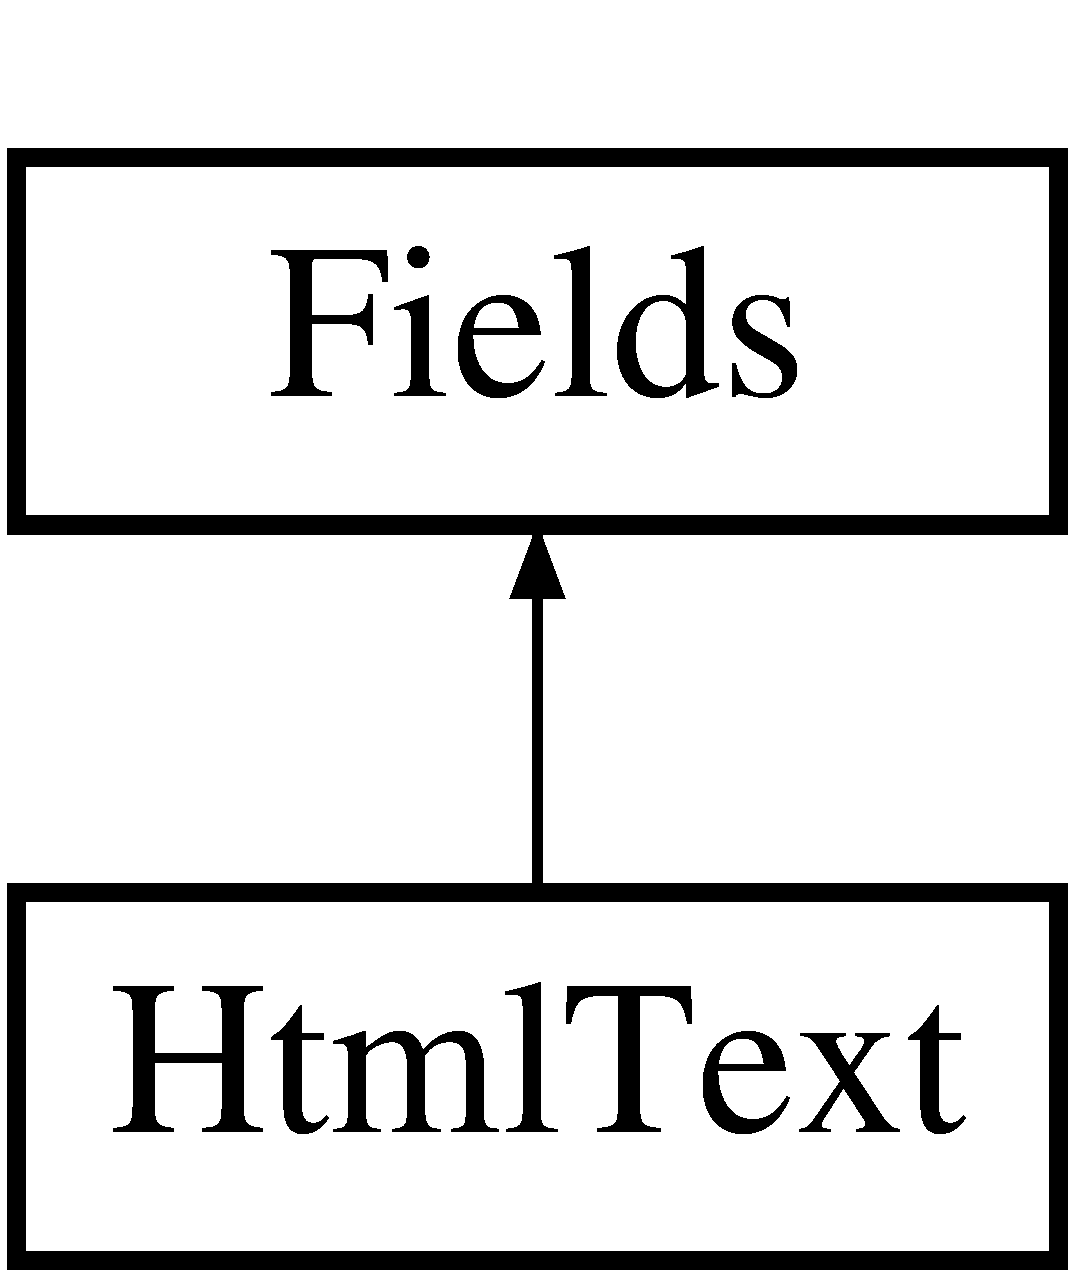
\includegraphics[height=2.000000cm]{class_html_text}
\end{center}
\end{figure}
\subsection*{Public Member Functions}
\begin{DoxyCompactItemize}
\item 
\hyperlink{class_html_text_ac610fc08cbb0781b26136636de129bc0}{\-\_\-\-\_\-construct} (\$nm)
\begin{DoxyCompactList}\small\item\em Constructor for class. \end{DoxyCompactList}\item 
\hypertarget{class_html_text_a421831a265621325e1fdd19aace0c758}{\hyperlink{class_html_text_a421831a265621325e1fdd19aace0c758}{\-\_\-\-\_\-destruct} ()}\label{class_html_text_a421831a265621325e1fdd19aace0c758}

\begin{DoxyCompactList}\small\item\em Default de-\/constructor for class. \end{DoxyCompactList}\item 
\hypertarget{class_html_text_a14814e04b348120748912692645f3a75}{\hyperlink{class_html_text_a14814e04b348120748912692645f3a75}{get\-Contents} ()}\label{class_html_text_a14814e04b348120748912692645f3a75}

\begin{DoxyCompactList}\small\item\em Get the value of the field as html format. Used by form. \end{DoxyCompactList}\end{DoxyCompactItemize}
\subsection*{Additional Inherited Members}


\subsection{Detailed Description}
Contains html text to output in \hyperlink{class_form}{Form}. 

Raw html can be stored and will out put accordingly. A very simple, yet elegant class. The text will output based on the order in which this field is added to the form. Only class that \hyperlink{class_form}{Form} will skip when returning array values. As such, \hyperlink{class_html_text}{Html\-Text} will not be saved into S\-Q\-L. Essentially, will be non-\/existent to the form class. If using this for formatting or css, refer to custom div settings for individual fields prior to using this \hyperlink{class_html_text}{Html\-Text}. 

\subsection{Constructor \& Destructor Documentation}
\hypertarget{class_html_text_ac610fc08cbb0781b26136636de129bc0}{\index{Html\-Text@{Html\-Text}!\-\_\-\-\_\-construct@{\-\_\-\-\_\-construct}}
\index{\-\_\-\-\_\-construct@{\-\_\-\-\_\-construct}!HtmlText@{Html\-Text}}
\subsubsection[{\-\_\-\-\_\-construct}]{\setlength{\rightskip}{0pt plus 5cm}\-\_\-\-\_\-construct (
\begin{DoxyParamCaption}
\item[{}]{\$nm}
\end{DoxyParamCaption}
)}}\label{class_html_text_ac610fc08cbb0781b26136636de129bc0}


Constructor for class. 

Requires unique name to be used in Forms. Nothing to do with fields or html attributes. There are none! 

The documentation for this class was generated from the following file\-:\begin{DoxyCompactItemize}
\item 
Form.\-php\end{DoxyCompactItemize}

\hypertarget{class_text_box}{\section{Text\-Box Class Reference}
\label{class_text_box}\index{Text\-Box@{Text\-Box}}
}


Text box field for \hyperlink{class_form}{Form}.  


Inheritance diagram for Text\-Box\-:\begin{figure}[H]
\begin{center}
\leavevmode
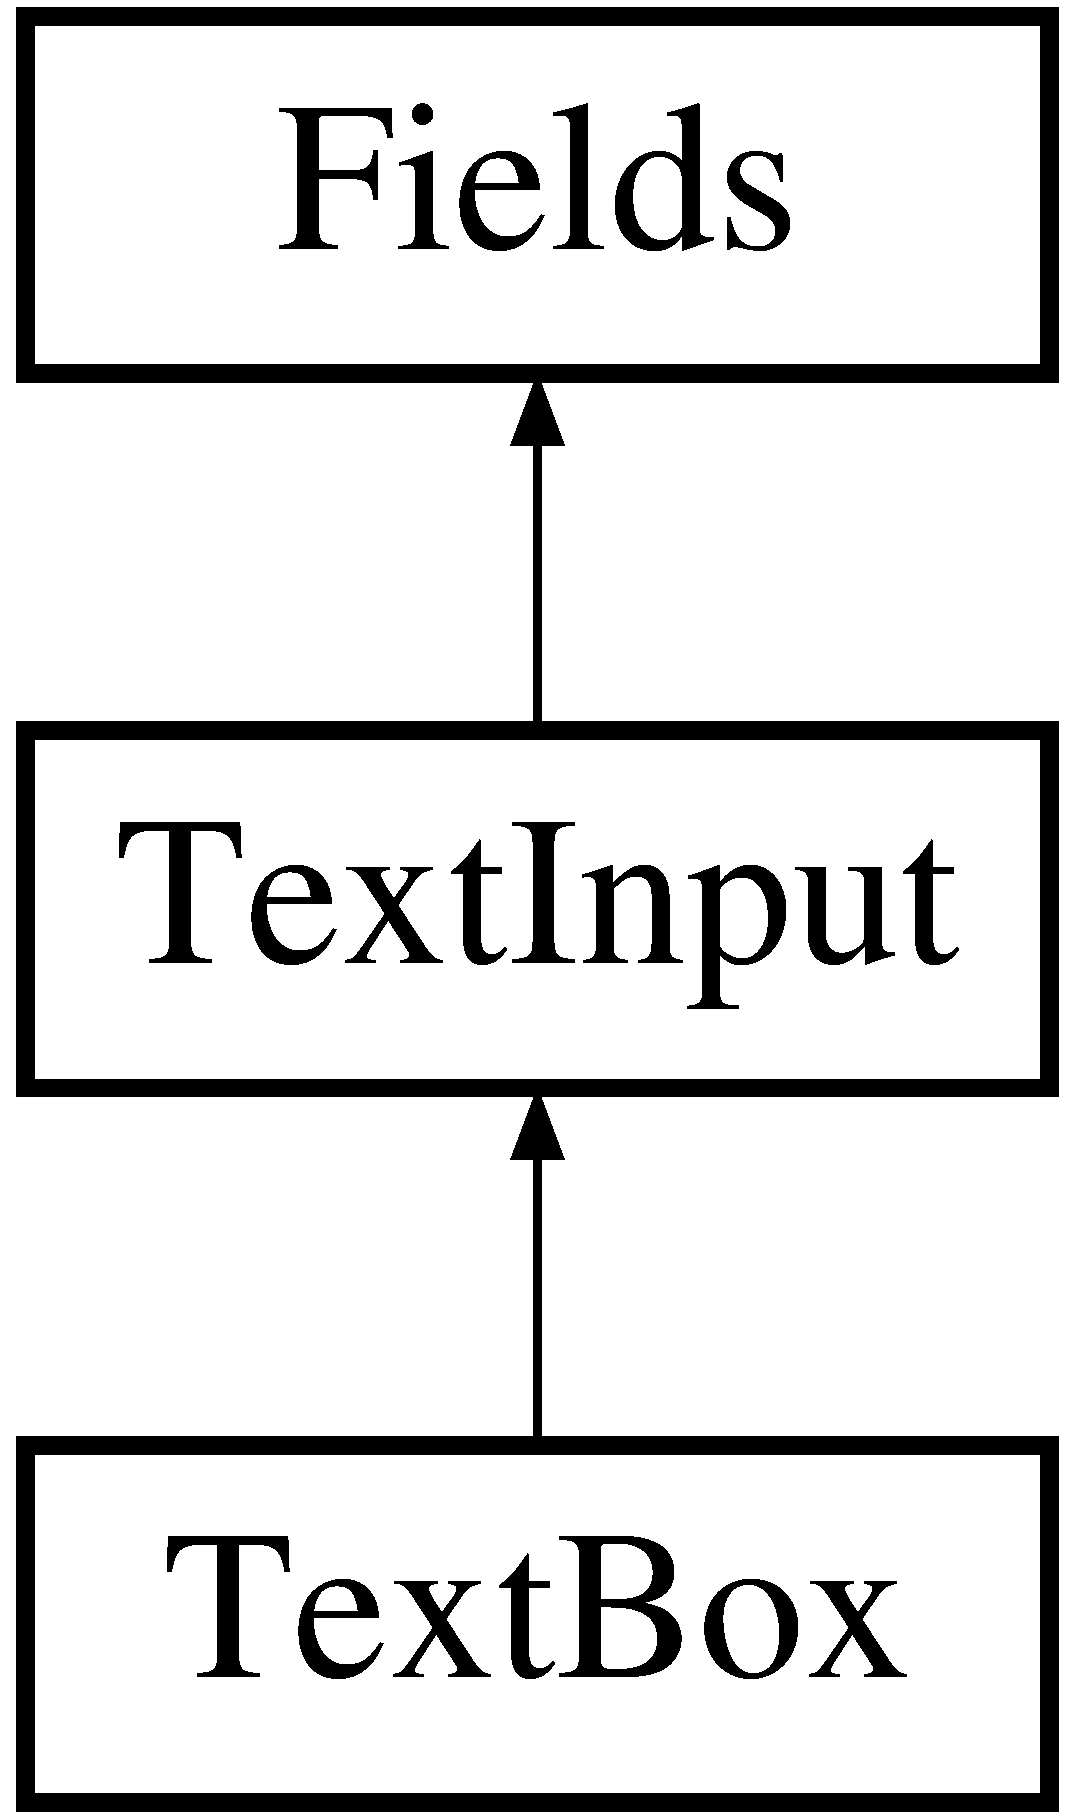
\includegraphics[height=3.000000cm]{class_text_box}
\end{center}
\end{figure}
\subsection*{Public Member Functions}
\begin{DoxyCompactItemize}
\item 
\hyperlink{class_text_box_ac610fc08cbb0781b26136636de129bc0}{\-\_\-\-\_\-construct} (\$nm)
\begin{DoxyCompactList}\small\item\em Constructor for class. \end{DoxyCompactList}\item 
\hypertarget{class_text_box_a14814e04b348120748912692645f3a75}{\hyperlink{class_text_box_a14814e04b348120748912692645f3a75}{get\-Contents} ()}\label{class_text_box_a14814e04b348120748912692645f3a75}

\begin{DoxyCompactList}\small\item\em Get the value of the field as html format. Used by form. \end{DoxyCompactList}\end{DoxyCompactItemize}
\subsection*{Additional Inherited Members}


\subsection{Detailed Description}
Text box field for \hyperlink{class_form}{Form}. 

Very much like \hyperlink{class_text_input}{Text\-Input}, as such, extends from it. Will need to add a height adjustment variables. 

\subsection{Constructor \& Destructor Documentation}
\hypertarget{class_text_box_ac610fc08cbb0781b26136636de129bc0}{\index{Text\-Box@{Text\-Box}!\-\_\-\-\_\-construct@{\-\_\-\-\_\-construct}}
\index{\-\_\-\-\_\-construct@{\-\_\-\-\_\-construct}!TextBox@{Text\-Box}}
\subsubsection[{\-\_\-\-\_\-construct}]{\setlength{\rightskip}{0pt plus 5cm}\-\_\-\-\_\-construct (
\begin{DoxyParamCaption}
\item[{}]{\$nm}
\end{DoxyParamCaption}
)}}\label{class_text_box_ac610fc08cbb0781b26136636de129bc0}


Constructor for class. 

Requires unique name to be used in field, html name attribute, and Forms. 

The documentation for this class was generated from the following file\-:\begin{DoxyCompactItemize}
\item 
Form.\-php\end{DoxyCompactItemize}

\hypertarget{class_text_input}{\section{Text\-Input Class Reference}
\label{class_text_input}\index{Text\-Input@{Text\-Input}}
}


Text input bar field for \hyperlink{class_form}{Form}.  


Inheritance diagram for Text\-Input\-:\begin{figure}[H]
\begin{center}
\leavevmode
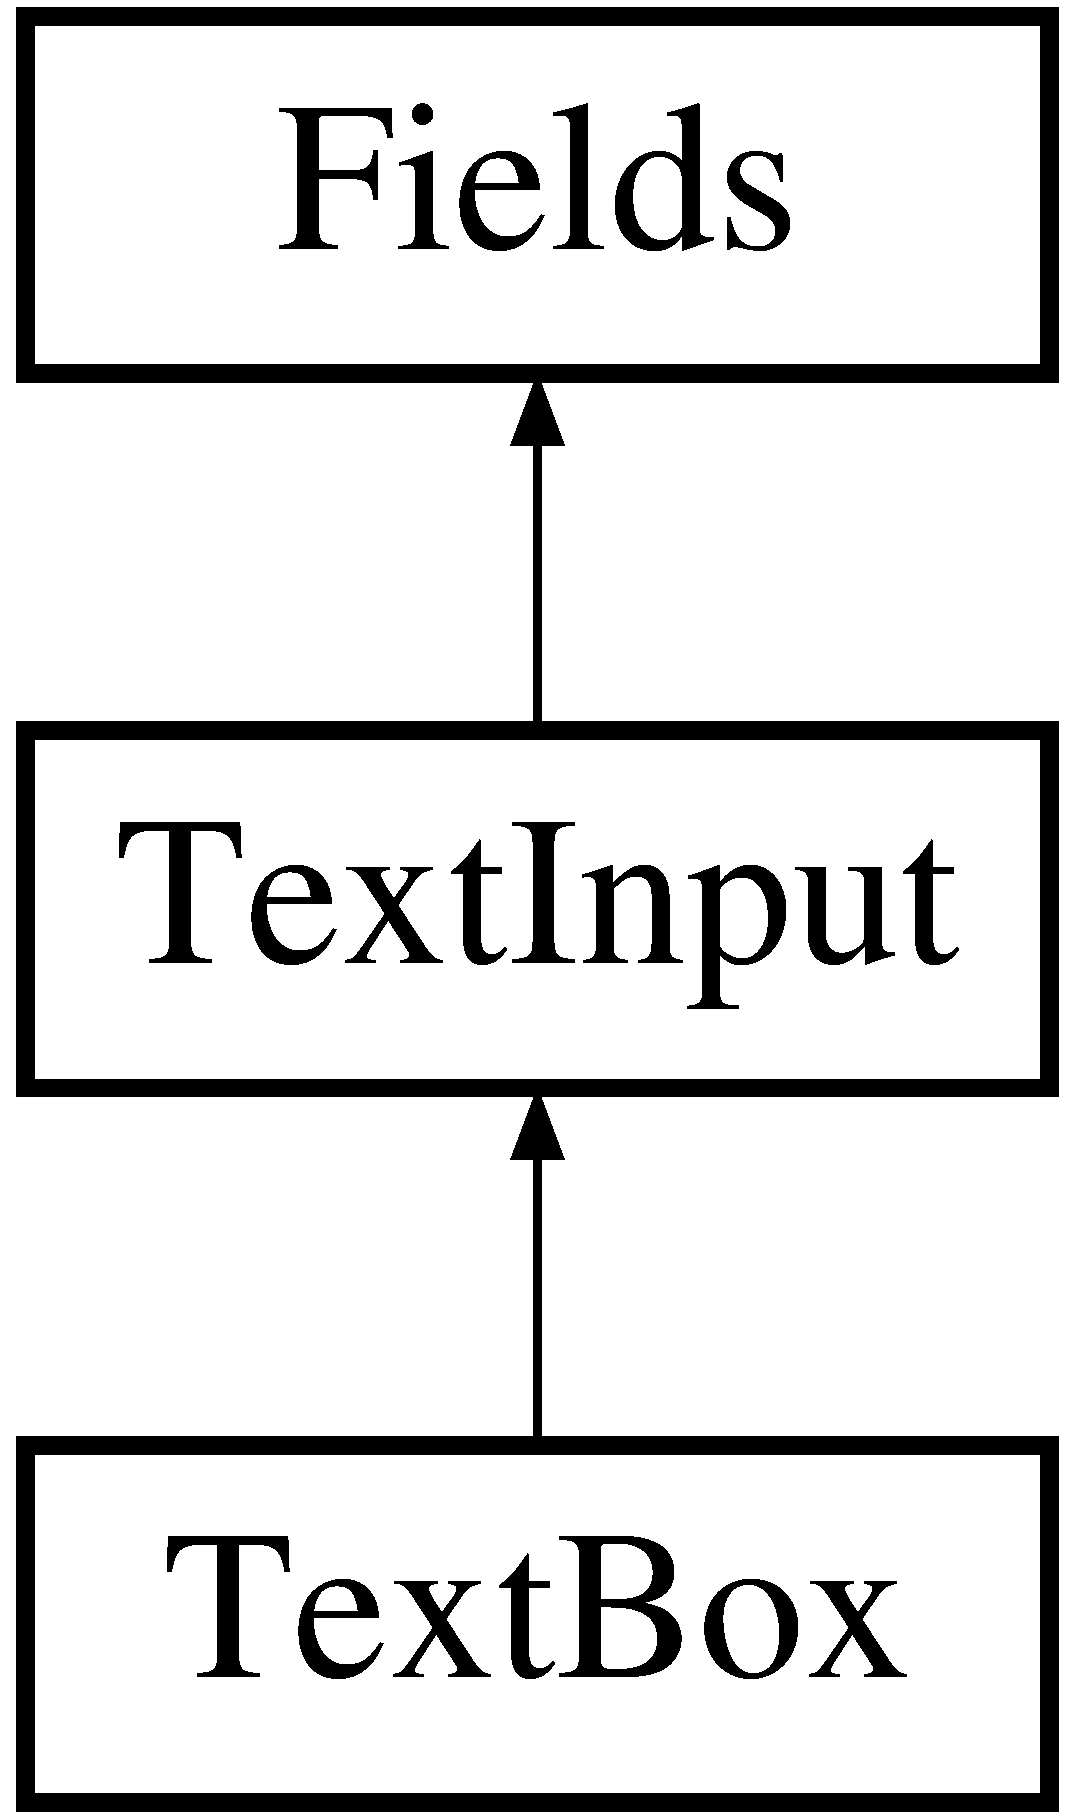
\includegraphics[height=3.000000cm]{class_text_input}
\end{center}
\end{figure}
\subsection*{Public Member Functions}
\begin{DoxyCompactItemize}
\item 
\hypertarget{class_text_input_a14814e04b348120748912692645f3a75}{\hyperlink{class_text_input_a14814e04b348120748912692645f3a75}{get\-Contents} ()}\label{class_text_input_a14814e04b348120748912692645f3a75}

\begin{DoxyCompactList}\small\item\em Get the value of the field as html format. Used by form. \end{DoxyCompactList}\item 
\hypertarget{class_text_input_a342df365ed03aee6a74989a388dff8c9}{\hyperlink{class_text_input_a342df365ed03aee6a74989a388dff8c9}{set\-Size} (\$s)}\label{class_text_input_a342df365ed03aee6a74989a388dff8c9}

\begin{DoxyCompactList}\small\item\em Set size or length of the input bar. Note\-: Height is not affected. \end{DoxyCompactList}\item 
\hyperlink{class_text_input_aef96c9ec2037beea335cd47fe7978bcc}{set\-Disabled} (\$d)
\begin{DoxyCompactList}\small\item\em Set if the input bar is locked. \end{DoxyCompactList}\item 
\hypertarget{class_text_input_acb30698aae42539e2b9ea3f6d172ce46}{\hyperlink{class_text_input_acb30698aae42539e2b9ea3f6d172ce46}{get\-Disabled} ()}\label{class_text_input_acb30698aae42539e2b9ea3f6d172ce46}

\begin{DoxyCompactList}\small\item\em Get boolean on if the input bar is locked. \end{DoxyCompactList}\end{DoxyCompactItemize}
\subsection*{Private Attributes}
\begin{DoxyCompactItemize}
\item 
\hypertarget{class_text_input_af594986e4618a8d6a5d7566617f583c6}{{\bfseries \$size} = 10}\label{class_text_input_af594986e4618a8d6a5d7566617f583c6}

\item 
\hypertarget{class_text_input_a6c108f5b26242d862f6e51869fbfd271}{{\bfseries \$disabled}}\label{class_text_input_a6c108f5b26242d862f6e51869fbfd271}

\end{DoxyCompactItemize}
\subsection*{Additional Inherited Members}


\subsection{Detailed Description}
Text input bar field for \hyperlink{class_form}{Form}. 

The most used class for field. It is simple in code as it only manages one data value. Refer to \hyperlink{class_text_box}{Text\-Box} for words longer than 5. (Note\-: May be exceptions) 

\subsection{Member Function Documentation}
\hypertarget{class_text_input_aef96c9ec2037beea335cd47fe7978bcc}{\index{Text\-Input@{Text\-Input}!set\-Disabled@{set\-Disabled}}
\index{set\-Disabled@{set\-Disabled}!TextInput@{Text\-Input}}
\subsubsection[{set\-Disabled}]{\setlength{\rightskip}{0pt plus 5cm}set\-Disabled (
\begin{DoxyParamCaption}
\item[{}]{\$d}
\end{DoxyParamCaption}
)}}\label{class_text_input_aef96c9ec2037beea335cd47fe7978bcc}


Set if the input bar is locked. 

Please note that when the input is locked, \$\-\_\-\-P\-O\-S\-T will not contain this variables. This means that \hyperlink{class_form}{Form} will not being able to read this info when passing \$\-\_\-\-P\-O\-S\-T directly to \hyperlink{class_form_a0fc192b82e0cc5ddfeb120046d3fff36}{Form\-::set\-Array\-Value}(\$post). As such, if you want to modify the value displayed in lock form, \hyperlink{class_fields_a013b668cd0771a560d9f8dd061badb82}{Fields\-::set\-Overide\-Def}(\$overide) may be used. 

The documentation for this class was generated from the following file\-:\begin{DoxyCompactItemize}
\item 
Form.\-php\end{DoxyCompactItemize}

\hypertarget{class_time_list}{\section{Time\-List Class Reference}
\label{class_time_list}\index{Time\-List@{Time\-List}}
}


A special drop list for time to be used in \hyperlink{class_form}{Form}.  


Inheritance diagram for Time\-List\-:\begin{figure}[H]
\begin{center}
\leavevmode
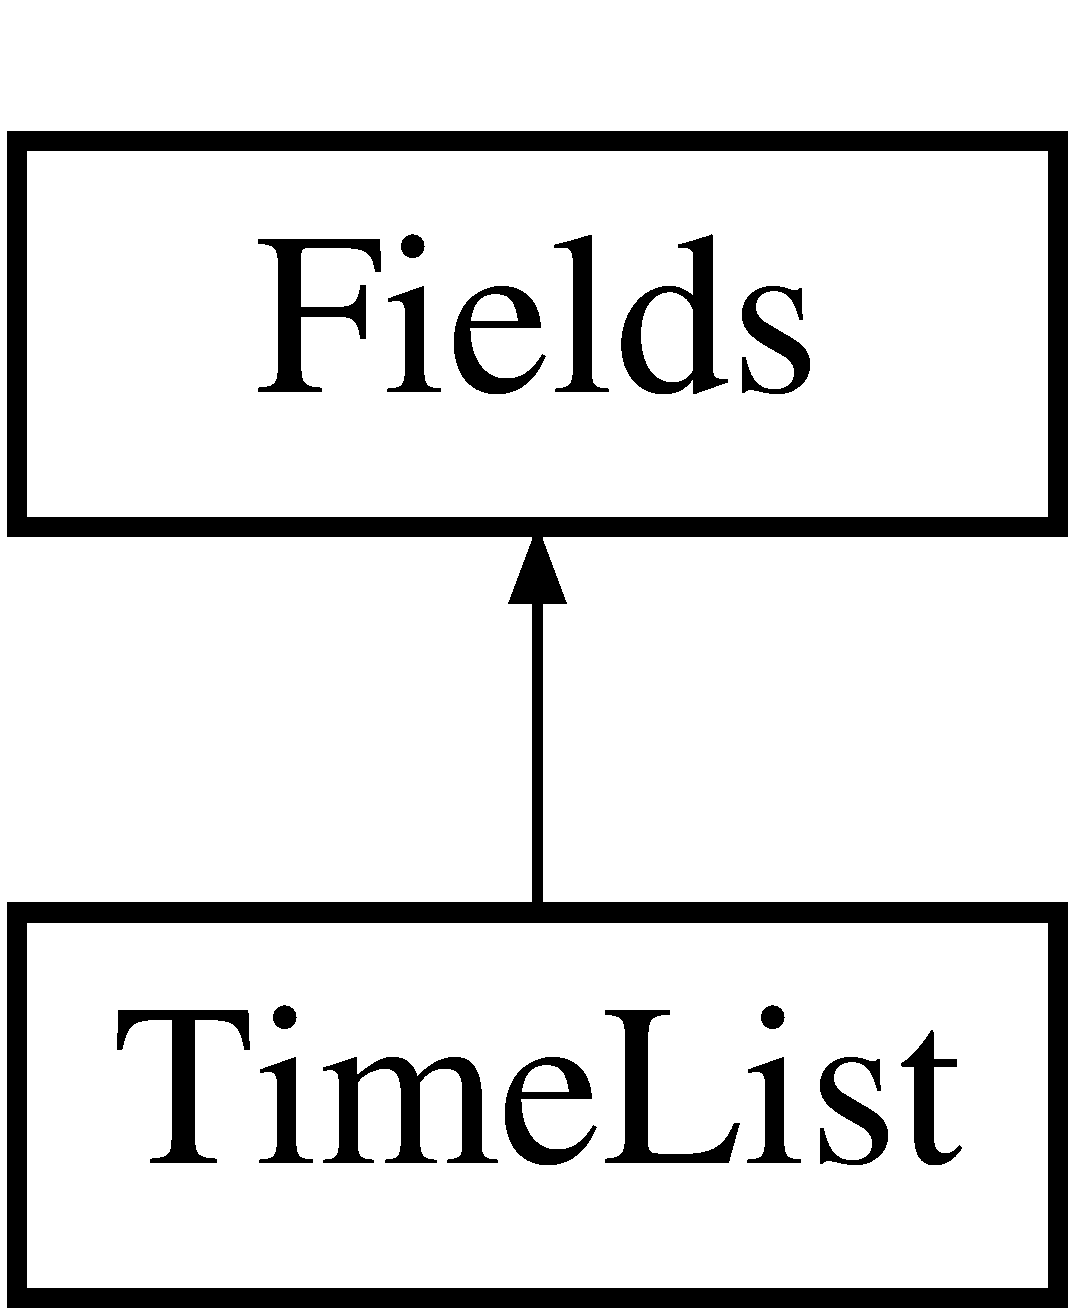
\includegraphics[height=2.000000cm]{class_time_list}
\end{center}
\end{figure}
\subsection*{Public Member Functions}
\begin{DoxyCompactItemize}
\item 
\hyperlink{class_time_list_ac610fc08cbb0781b26136636de129bc0}{\-\_\-\-\_\-construct} (\$nm)
\begin{DoxyCompactList}\small\item\em Constructor for class. \end{DoxyCompactList}\item 
\hypertarget{class_time_list_a421831a265621325e1fdd19aace0c758}{\hyperlink{class_time_list_a421831a265621325e1fdd19aace0c758}{\-\_\-\-\_\-destruct} ()}\label{class_time_list_a421831a265621325e1fdd19aace0c758}

\begin{DoxyCompactList}\small\item\em Default de-\/constructor for class. \end{DoxyCompactList}\item 
\hyperlink{class_time_list_aaf2bb7deba74bb0f994044954bd74ff3}{set\-Default} (\$d)
\begin{DoxyCompactList}\small\item\em Set default of \hyperlink{class_time_list}{Time\-List}. \end{DoxyCompactList}\item 
\hyperlink{class_time_list_a14814e04b348120748912692645f3a75}{get\-Contents} ()
\begin{DoxyCompactList}\small\item\em Get the value of the field as html format. Used by form. \end{DoxyCompactList}\item 
\hypertarget{class_time_list_a6f75ffe7d98c9e375394d63f8d379b2d}{{\bfseries set\-Class} (\$nm)}\label{class_time_list_a6f75ffe7d98c9e375394d63f8d379b2d}

\item 
\hypertarget{class_time_list_a4e25c00802ca9e9afb52a9177014fea7}{{\bfseries set\-Div\-Class} (\$nm)}\label{class_time_list_a4e25c00802ca9e9afb52a9177014fea7}

\end{DoxyCompactItemize}
\subsection*{Private Member Functions}
\begin{DoxyCompactItemize}
\item 
\hypertarget{class_time_list_adb57b56db9f1cbbe4e72ed05e2d5bd8a}{{\bfseries format\-List} (\$nm)}\label{class_time_list_adb57b56db9f1cbbe4e72ed05e2d5bd8a}

\end{DoxyCompactItemize}
\subsection*{Additional Inherited Members}


\subsection{Detailed Description}
A special drop list for time to be used in \hyperlink{class_form}{Form}. 

Supports up to an hour of time. If more, normal lists should be used. This was used for special cases where formatting of time is of an issue. Much like \hyperlink{class_date_list}{Date\-List} where multiple \hyperlink{class_drop_list}{Drop\-List} are created and managed. 

\subsection{Constructor \& Destructor Documentation}
\hypertarget{class_time_list_ac610fc08cbb0781b26136636de129bc0}{\index{Time\-List@{Time\-List}!\-\_\-\-\_\-construct@{\-\_\-\-\_\-construct}}
\index{\-\_\-\-\_\-construct@{\-\_\-\-\_\-construct}!TimeList@{Time\-List}}
\subsubsection[{\-\_\-\-\_\-construct}]{\setlength{\rightskip}{0pt plus 5cm}\-\_\-\-\_\-construct (
\begin{DoxyParamCaption}
\item[{}]{\$nm}
\end{DoxyParamCaption}
)}}\label{class_time_list_ac610fc08cbb0781b26136636de129bc0}


Constructor for class. 

Requires unique name to be used in field, html name attribute, and Forms. 

\subsection{Member Function Documentation}
\hypertarget{class_time_list_a14814e04b348120748912692645f3a75}{\index{Time\-List@{Time\-List}!get\-Contents@{get\-Contents}}
\index{get\-Contents@{get\-Contents}!TimeList@{Time\-List}}
\subsubsection[{get\-Contents}]{\setlength{\rightskip}{0pt plus 5cm}get\-Contents (
\begin{DoxyParamCaption}
{}
\end{DoxyParamCaption}
)}}\label{class_time_list_a14814e04b348120748912692645f3a75}


Get the value of the field as html format. Used by form. 

Individual \hyperlink{class_drop_list}{Drop\-List} html names are\-: \$this-\/$>$name.'sec' and \$this-\/$>$name.'min'. \hypertarget{class_time_list_aaf2bb7deba74bb0f994044954bd74ff3}{\index{Time\-List@{Time\-List}!set\-Default@{set\-Default}}
\index{set\-Default@{set\-Default}!TimeList@{Time\-List}}
\subsubsection[{set\-Default}]{\setlength{\rightskip}{0pt plus 5cm}set\-Default (
\begin{DoxyParamCaption}
\item[{}]{\$d}
\end{DoxyParamCaption}
)}}\label{class_time_list_aaf2bb7deba74bb0f994044954bd74ff3}


Set default of \hyperlink{class_time_list}{Time\-List}. 

Must be formatted as '00m 00s' with a space. 

The documentation for this class was generated from the following file\-:\begin{DoxyCompactItemize}
\item 
Form.\-php\end{DoxyCompactItemize}

%--- End generated contents ---

% Index
\newpage
\phantomsection
\addcontentsline{toc}{chapter}{Index}
\printindex

\end{document}
